\documentclass[a4, 10pt, twoside, twocolumn]{article}

\usepackage[hidelinks]{hyperref}
\usepackage{graphicx}
\usepackage{caption}
\usepackage{subcaption}
\usepackage{afterpage}
\usepackage{fancyhdr}
\usepackage{geometry}
\usepackage{pdflscape}
\usepackage[toc,page]{appendix}
\usepackage{amsmath}
\usepackage{listings}
\usepackage{color} %red, green, blue, yellow, cyan, magenta, black, white
\definecolor{mygreen}{RGB}{28,172,0} % color values Red, Green, Blue
\definecolor{mylilas}{RGB}{170,55,241}

\numberwithin{figure}{section}
\pagestyle{fancy}
\fancyfoot{} % clear all footer fields
\fancyfoot[LE,RO]{\thepage}
\fancypagestyle{plain}
{
    \renewcommand{\headrulewidth}{0pt}%
    \fancyhead{}
    \fancyhead[R]{attn. Prof.\,dr.\,ir.\,Johan Suykens}
    \fancyfoot[R]{\thepage}
}

\begin{document}

\title
{
	[H02C4A] Artificial Neural Networks\\
	Report on exercises and projects
}
\author
{
    Sven Van Hove (s0190440)\\
    Program: credit contract
}
\date{2016 -- 2017}

\maketitle

\section{Supervised learning and generalization}

In this exercise, a feedforward neural network with one input (excl. bias), one hidden layer and one output neuron is used to approximate two periods of a sine wave. Given sufficient hidden neurons, this should not pose any problems because neural nets are universal approximators. Hornik's theorem states that a neural network with one hidden layer can approximate any continous function arbitrarily well.

The effect on network performance of various parameters combinations including train function, number of hidden neurons, noise level and number of training samples are evaluated. Default values will be used for all other parameters such as the transfer function, the learn function and parameters specific to the train function. The following train functions are included in the test set: \texttt{traingd}, \texttt{traingda}, \texttt{traincgf}, \texttt{traincgp}, \texttt{trainbfg}, \texttt{trainlm} and \texttt{trainbr}. Other predefined train functions exist, but those are beyond the scope of this report. Regarding the number of hidden neurons, the minimum amount used is 5 because preliminary tests indicated that this architecture can consistently (i.e. at least in ten consecutive runs) represent two periods of a sine wave faithfully with default parameters. Note that more neurons are required if more periods of the wave need to be approximated, meaning that the network does not learn the periodic nature of the input. Other tests use 10, 15, 20 and 100 neurons in the hidden layer. The noise level superimposed on the training data (expressed as the standard deviation $\sigma$ of Gaussian noise) starts at zero, but is increased in steps of 0.1 to 0.4 in subsequent tests. Finally, the number of training data is determined indirectly by the step size used for the input vector of the sine wave.

Network performance is measured in terms of correctness, speed, overfitting and generalization. Due to the non-determinism of some steps in the process (in particular weights and bias initialization and train/validation/test divisions), each test will be repeated ten times and aggregated statistics will be reported. Correctness will be stated in terms of the regression R value. Note that a high R value alone does not guarantee a good fit. The residuals should not exhibit any pattern; ideally they are random noise. Speed will be measured with the MATLAB tic-toc functions. Overfitting only becomes an issue when noise is added to the training data. In that case, the network should ideally be able to approximate the underlying sine wave, while ignoring the noise.
%R = which is a measure of the amount of variability in the input data that can be explained by the neural network

\afterpage{\begin{landscape}
    \thispagestyle{empty}
    \begin{figure}[p]
        \begin{subfigure}{0.37\linewidth}
            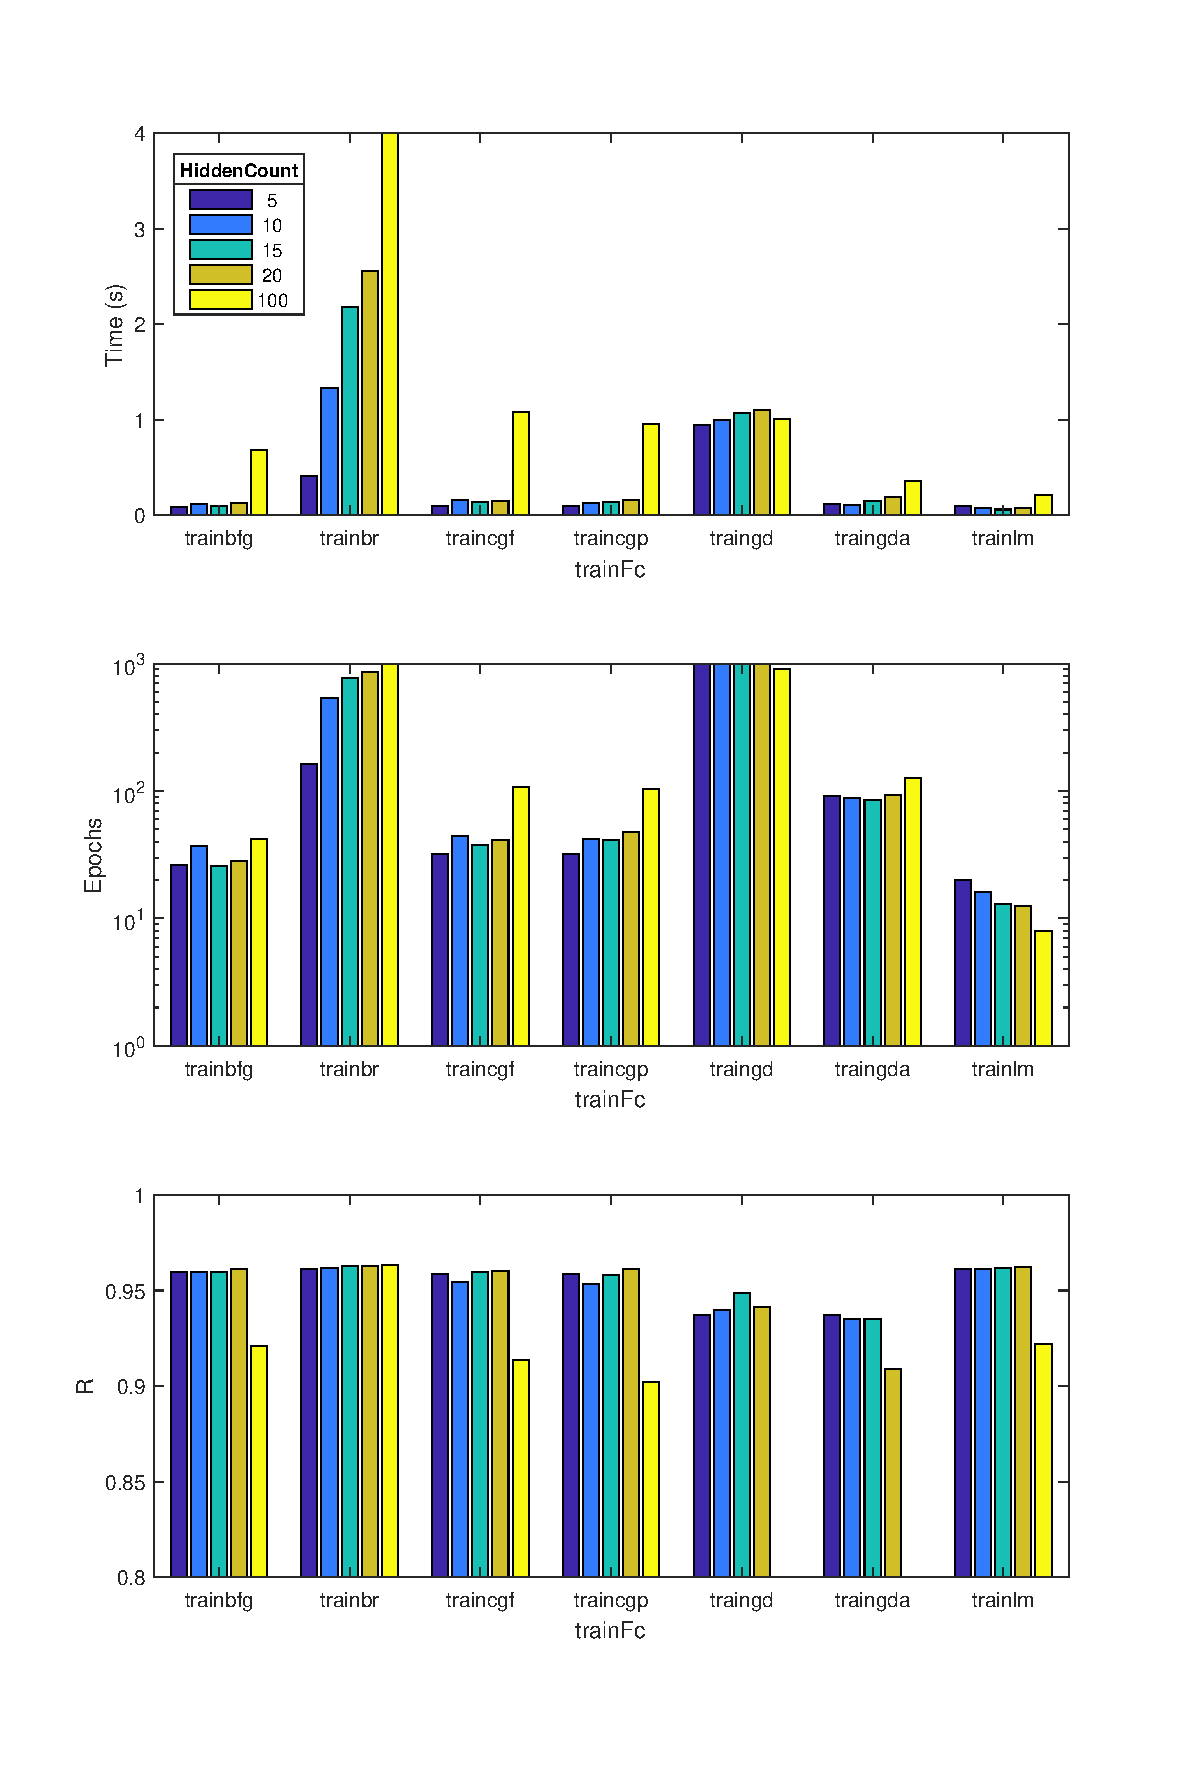
\includegraphics[width=\linewidth]{img/HiddenCount.pdf}
            \caption{Number of hidden neurons}
        \end{subfigure}
        \begin{subfigure}{0.37\linewidth}
            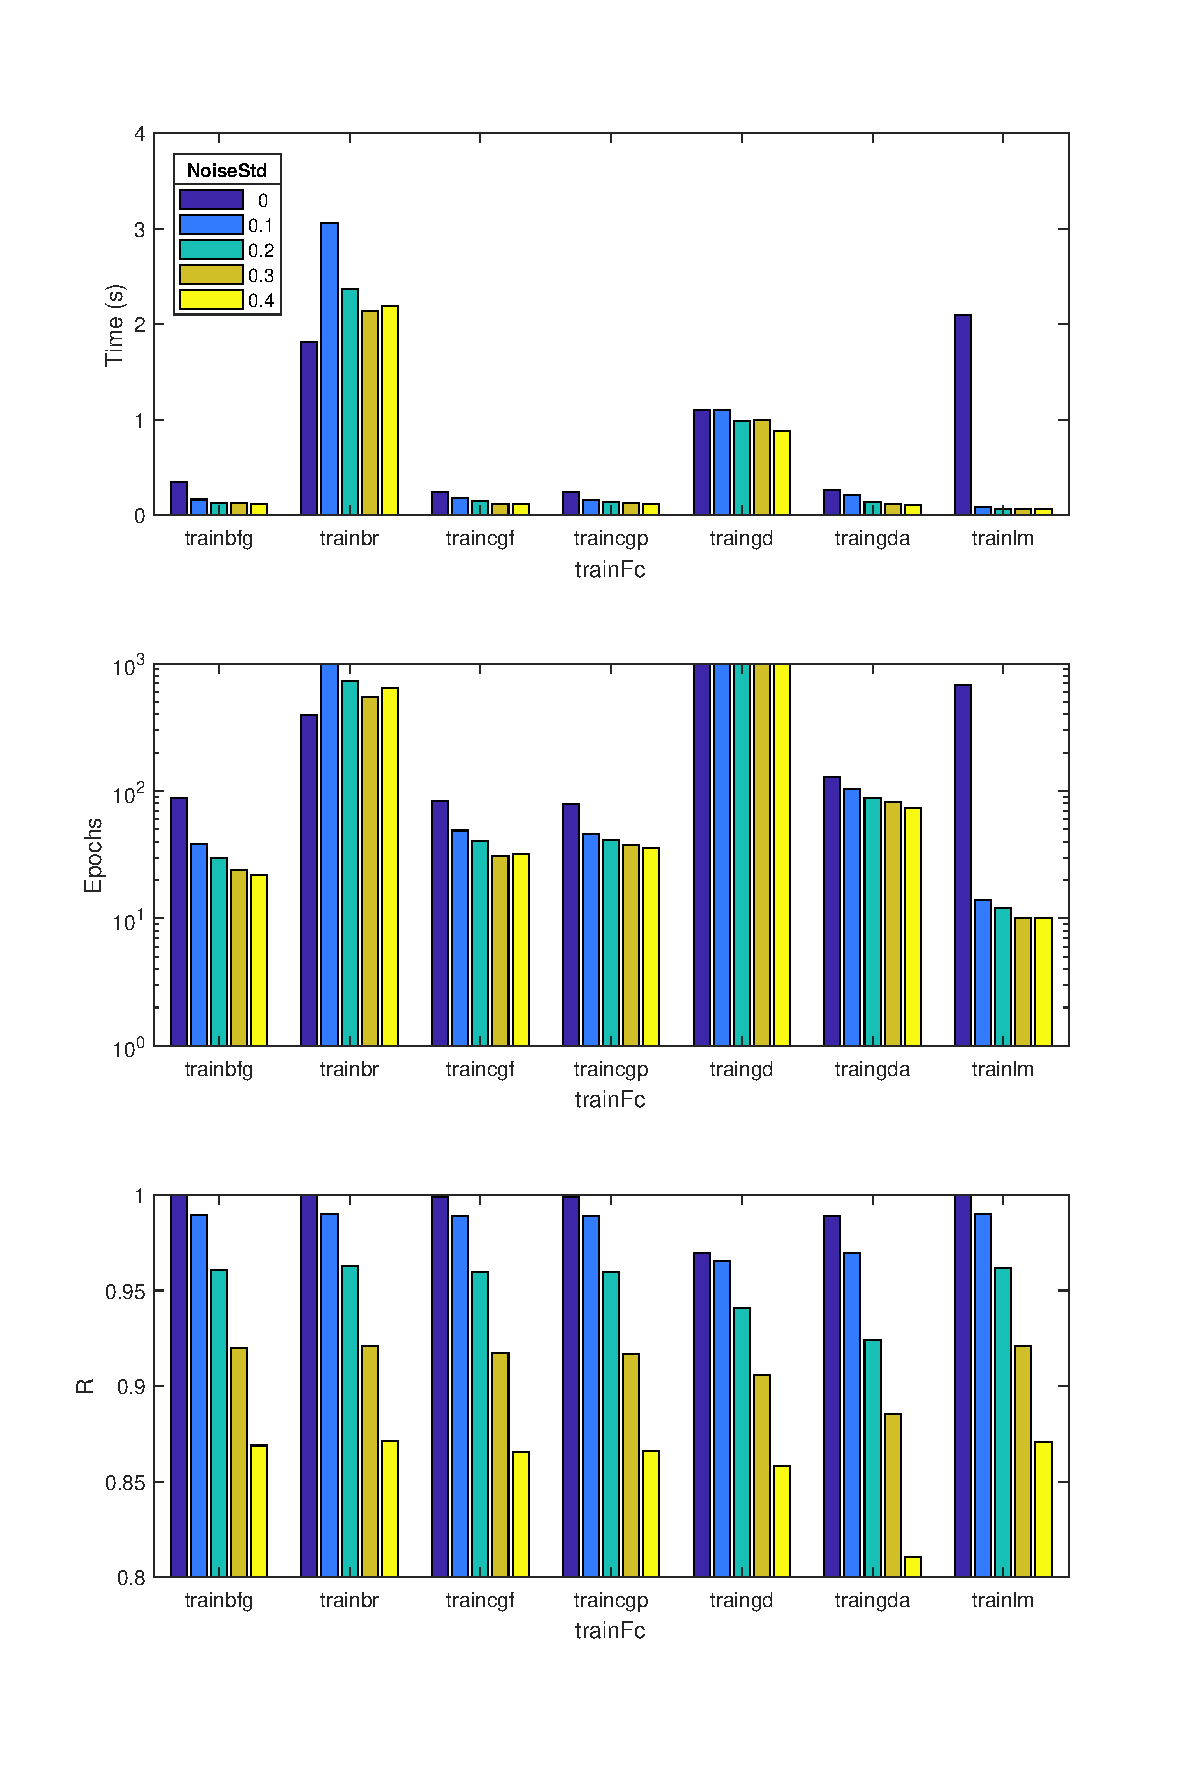
\includegraphics[width=\linewidth]{img/NoiseStd.pdf}
            \caption{Noise $\sigma$}
        \end{subfigure}
        \begin{subfigure}{0.37\linewidth}
            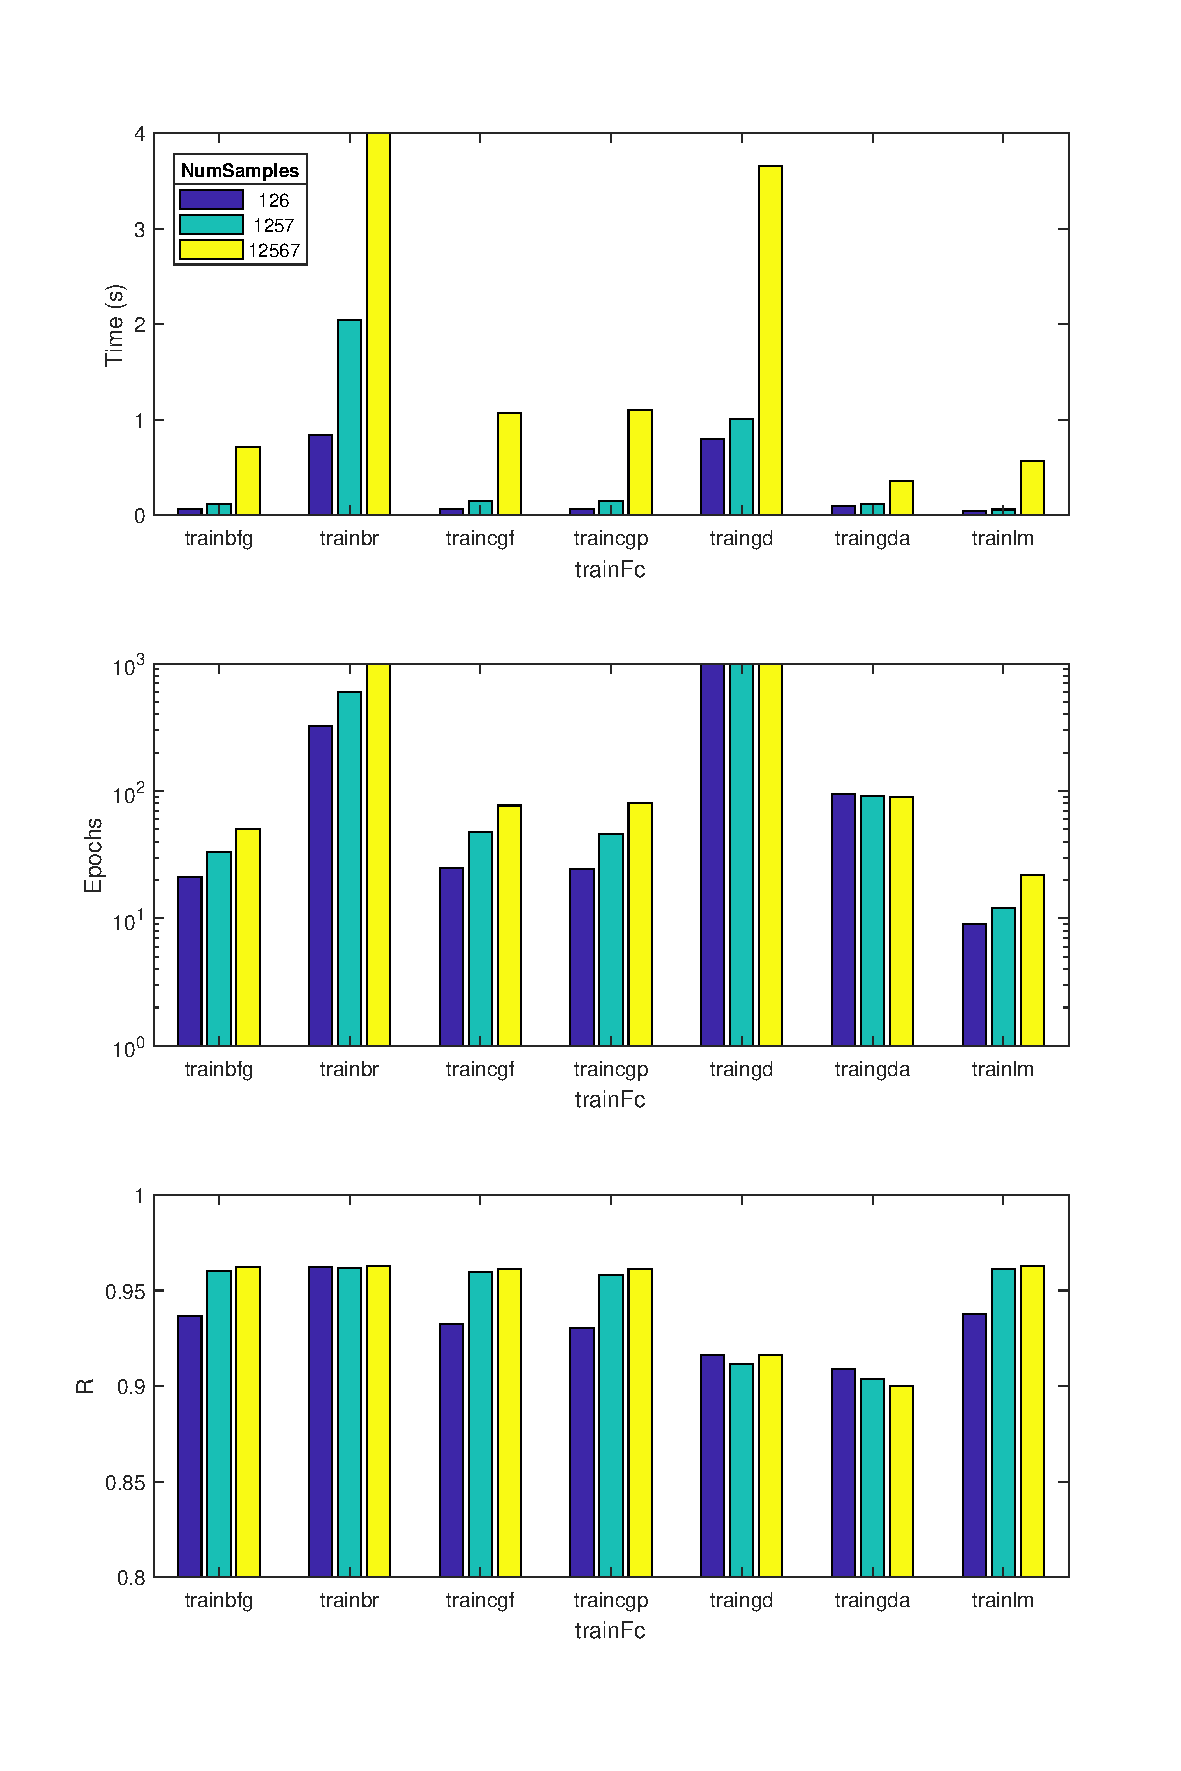
\includegraphics[width=\linewidth]{img/NumSamples.pdf}
            \caption{Number of samples}
        \end{subfigure}
        \caption{Effect of various parameters on network performs in terms of train time, number of epochs and R value.}
        \label{fig:results}
    \end{figure}
\end{landscape}}

The results are summarized in \autoref{fig:results}. The first thing to note is that raising the number of hidden neurons in most cases increases training time - especially for \texttt{trainbr} (up to 98s) - while it does not increase the R value significantly. For overparametrized networks with hundred hidden neurons, the R values are typically much lower. The optimization problem becomes undercharacterized because there are many more weights to adjust, yet not enough training samples to constrain them. Furthermore, more hidden neurons means more flexibility, which can encourage overfitting. The only exception is once again \texttt{trainbr}, but the increased time makes this a poor trade-off. Another finding is that \texttt{trainlm} is a very fast algorithm that manages to generate very good R values. The downside is that it requires more memory than other training functions (MATLAB approximates the Hessian with the Jacobian matrix) \cite{helptrainlm}.

Not surprisingly, raising the noise level lowers the R value of the regression between the network output and the noisy input. A network that generalizes well should instead aim for a perfect regression between network output and noiseless input. What is surprising, is that the train time lowers with increased noise - significantly so for \texttt{trainlm}.

Finally, increasing the number of training samples evidently increases training time and also R values, but only up to a certain point. Once enough information is available, additional samples are pure overhead for most training functions. Remarkably, \texttt{trainbr} scores well regardless of the number of training samples.

In general, \texttt{trainbfg}, \texttt{traincgf} and \texttt{traincgp} perform very similar but rarely as good as \texttt{trainlm}, while \texttt{traingd} and to a lesser extent \texttt{traingda} perform rather weak. \texttt{trainbr} is definitely the odd one out because the underlying algorithm is very different.

%TODO bias vs variance?
%TODO more detail trainbr?

\section{Recurrent neural nets}

\subsection{Hopfield network}
\label{ssec:hopfield}
In this exercise, a 240-neuron Hopfield recurrent network is used to perform digit recognition based on ten $15 \times 16$ binary images with values in $\{-1, 1\}$. The network is created in such a way that each of the ten digits is an attractor state. This is done by serializing each digit image to a 240D vector $d_i$ and initializing the network using those ten vectors. An energy field is created where the given attractors correspond to local minima.

A well known problem with Hopfield networks is the possible existence of spurious attractor states. These are also local minima in the energy field that behave exactly the same as traditional attractor states, but they are not explicitly provided during initialization. Consequently, in our example an input vector may converge to such a spurious attractor instead of to one of the ten digit vectors. Decoding a spurious attractor into a binary image will result in gibberish. Spurious attractors often appear on symmetry lines between other attractors or as the negation of another attractor. A strategic search using inputs $-d_i$ and $\frac{d_i + d_j}{2}$ for digits $i$ and $j$ revealed only one such spurious attractor. A brute force search with inputs consisting of pure noise revealed four more unique spurious attractors. All are shown in \autoref{fig:spurious}. It is remarkable how similar they are to the templates for digits two and seven. This could make their detection more difficult compared to other digits.

\begin{figure}[ht]
    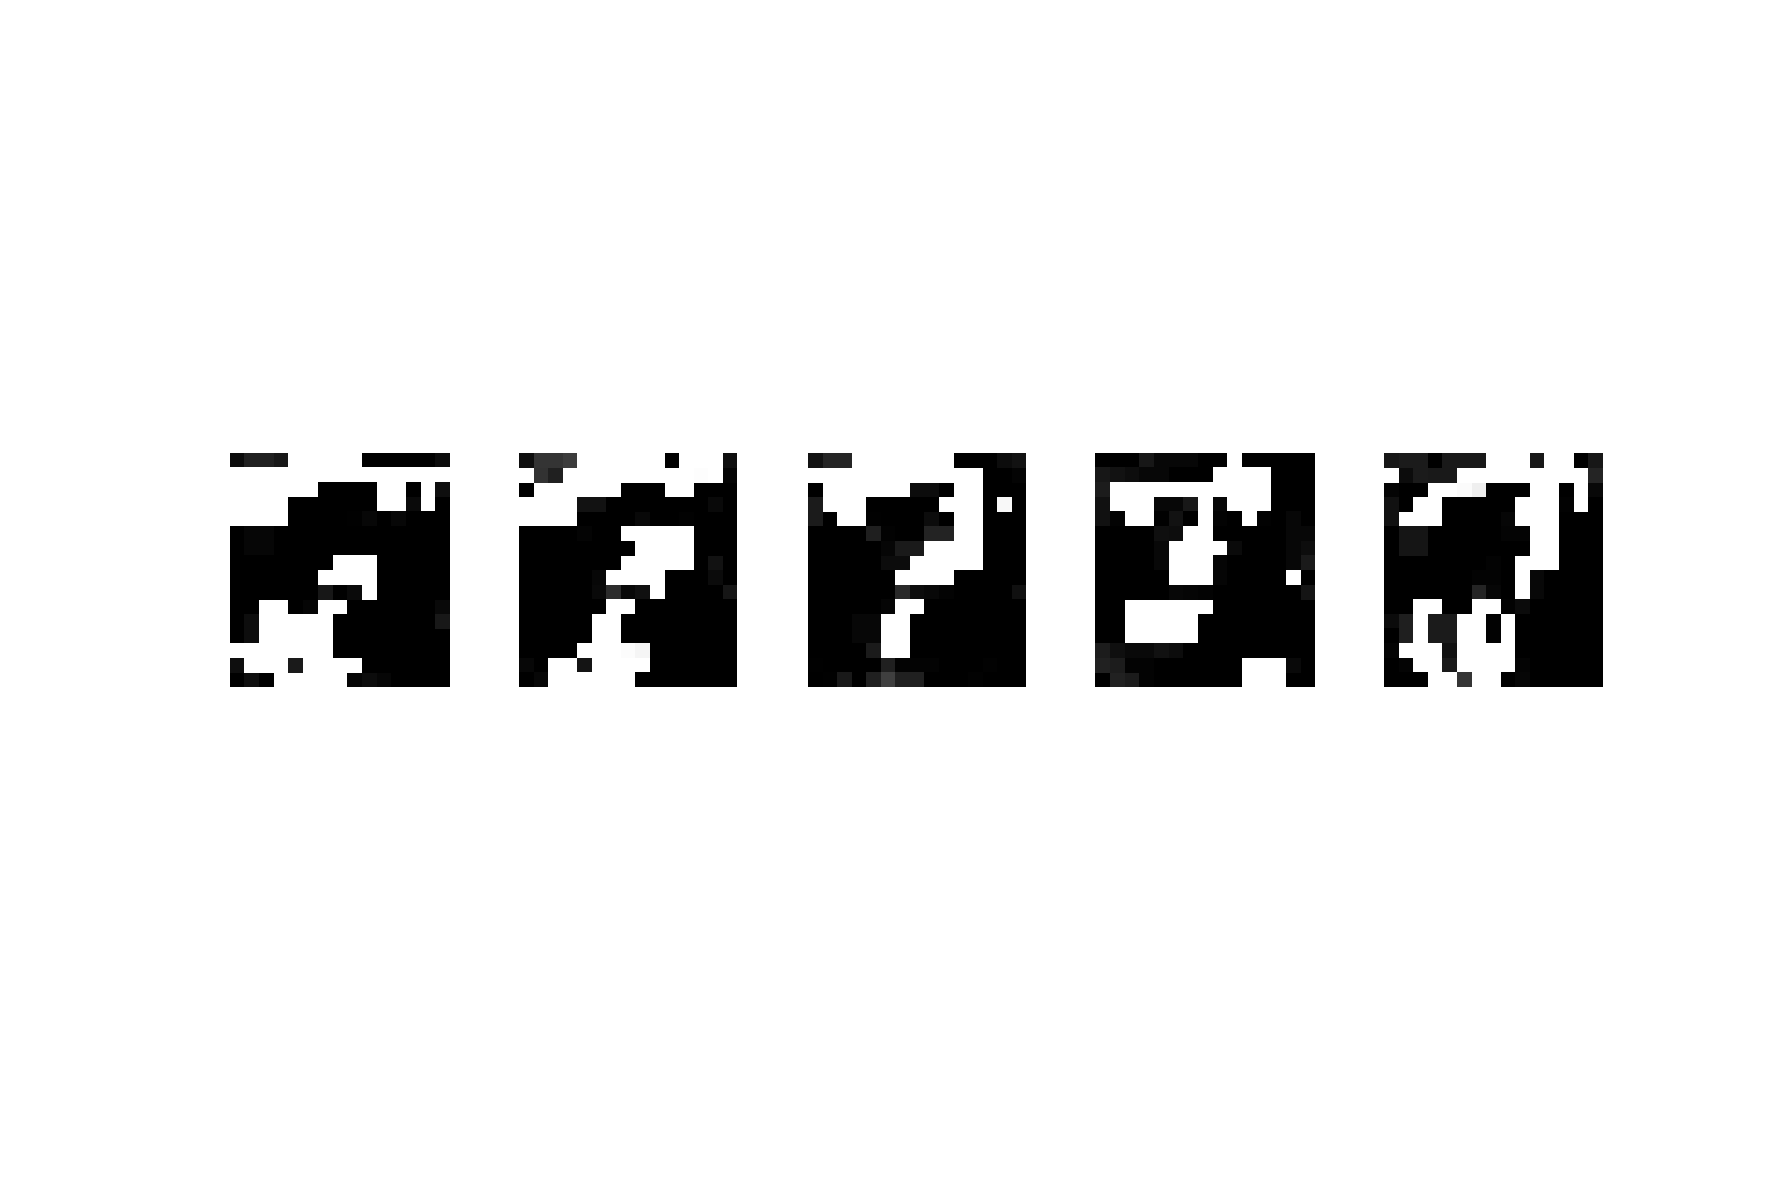
\includegraphics[width=\linewidth, trim=3cm 8cm 3cm 8cm, clip]{img/Spurious.pdf}
    \caption{Image representation of five spurious states.}
    \label{fig:spurious}
\end{figure}

Other problematic cases include when the network has not yet converged or when it did not converge to the expected digit. To test network resilience, the original digit images are corrupted by adding random noise of a given level $\sigma$. This noise will displace the vector in the 240D space. For high noise levels, the displacement could be so large that the vector leaves the basin of its local minimum in the energy field. The resulting vector will then converge to another attractor state, which may or may not be spurious. For $\sigma = 4$ (and 500 iterations), errors start to appear. Over 1000 trials with 10 digits each, 9415 samples were identified correctly. The minimum accuracy per digit was 916/1000 for digit eight while digit two scored highest with 960/1000. 16 samples failed to converge to the correct digit. Digits two, six and seven were responsible for most of these cases, with respective counts 5, 4 and 4. \autoref{fig:detect8} shows detailed results for digit eight.

\begin{figure}[ht]
    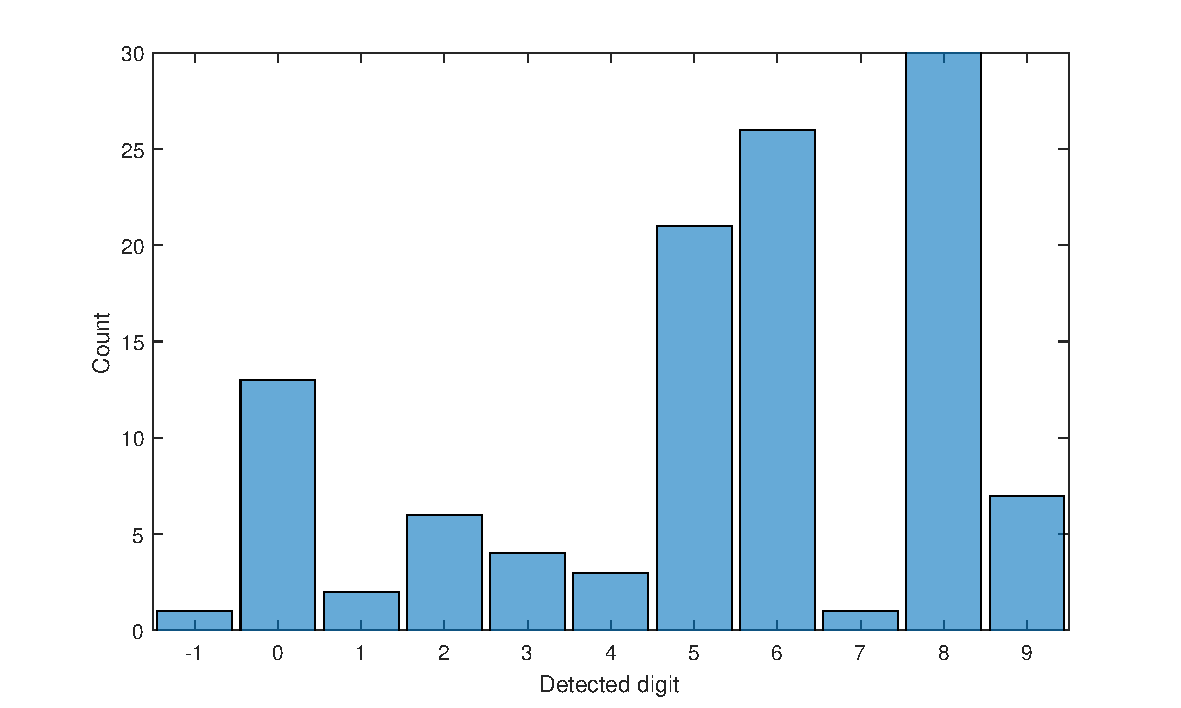
\includegraphics[width=\linewidth]{img/Detect8.pdf}
    \caption{Results over 1000 trials for noisy inputs ($\sigma = 4$) of digit eight. Detected digit -1 signals a spurious result. The network most often mistakes digit eight for digit five or six.}
    \label{fig:detect8}
\end{figure}

More high level results for various noise levels and iteration counts can be found in \autoref{fig:EffectSigmaIterations}. If there is no noise, the number of successes is 100\% and there are no failures. High iteration levels ensure that almost all samples converge to a digit, but the higher the noise level the more likely the algorithm chooses the wrong digit.

\begin{figure}[ht]
    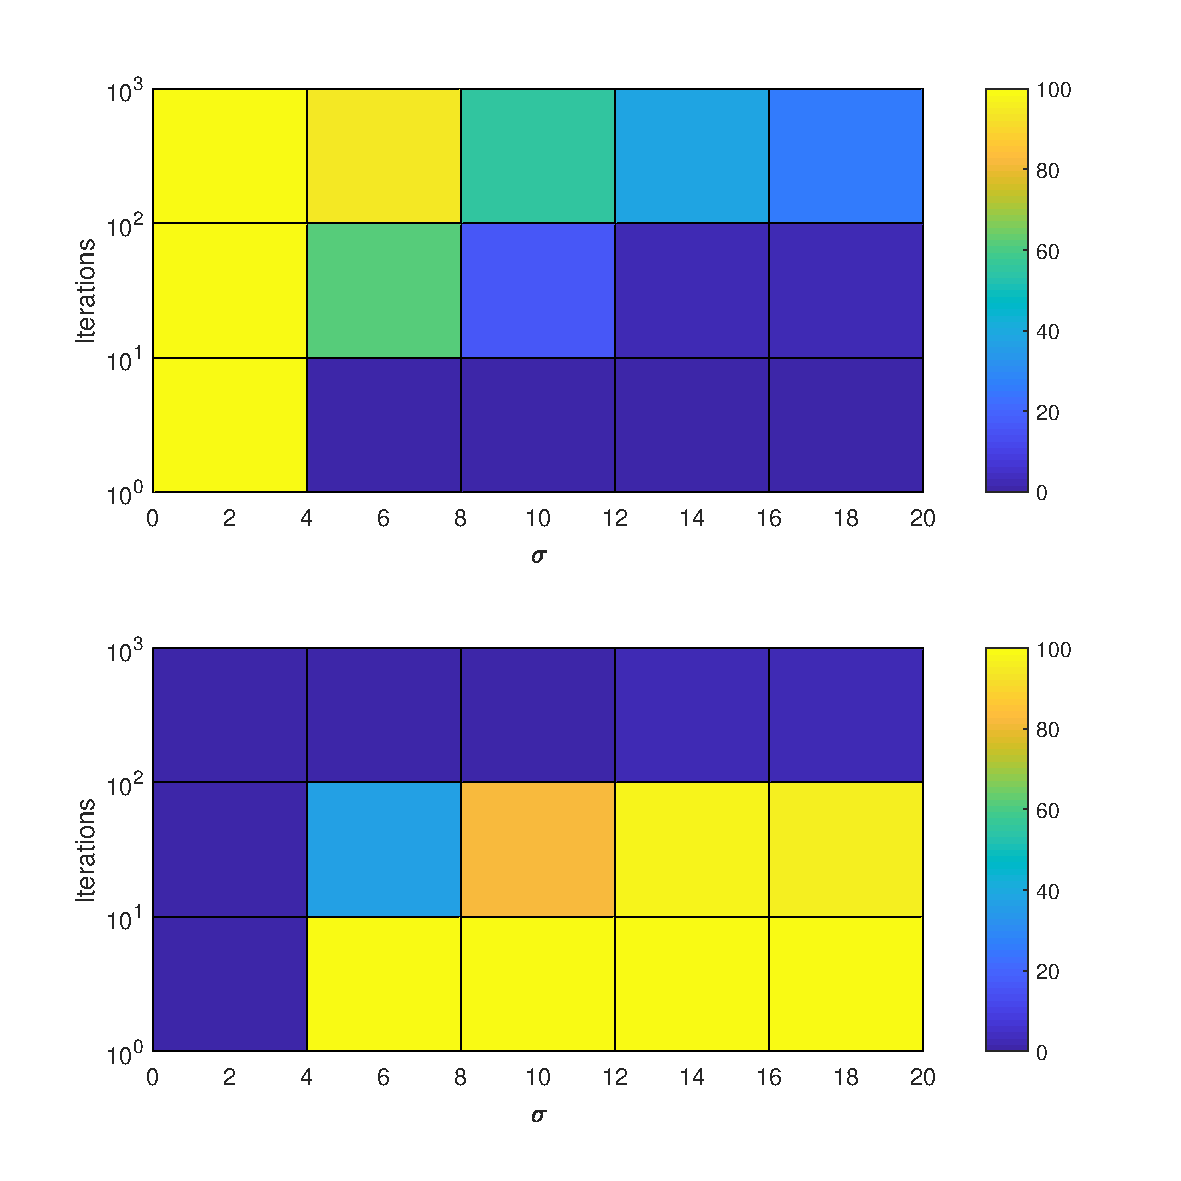
\includegraphics[width=\linewidth]{img/EffectSigmaIterations.pdf}
    \caption{Results over 10 trials with 10 digits each for noisy inputs with various $\sigma$ levels and iteration counts. Top: number of samples successfully retrieved. Bottom: number of samples that did not converge to a digit (i.e. not converged at all or converged to a spurious attractor). The number of samples that converged to a different digit is not shown but can easily be deduced as the sum of the three components must equal 1000.}
    \label{fig:EffectSigmaIterations}
\end{figure}

% Note that in the real world, the variation in handwritten digits between people is very different from the variation created by adding random noise to the original template. Regardless, if they remain close enough to the template in 240-dimensional space, Hopfield networks should be able to recognize them. The scans are also likely to be in higher resolution, but may be scaled down to reduce the required computational power.

\subsection{Elman network}
% nums_neurons = [1,2,3,4,5,10,15,20,25]; %50
% nums_samples = [100, 1000, 10000];
% nums_epochs = [10, 100, 1000];
% percs_train_val = 0.1:0.1:0.8; %300
% perc_training = 0.7;
% perc_test = 0.2; %200
% repeat = 10;

In this exercise, an Elman recurrent neural network is used to analyze the Hammerstein time series and make predictions. Various network architectures are tested, with 1 to 5 neurons and also 10 to 25 neurons in increments of 5. The total number of samples for training, validation and testing was 100, 1 000 or 10 000. Of this total, percentages between 10\% and 80\% with 10 percentpoint increments were used for training and validation while the last 20\% was used for testing. The training-validation split was constant at 70\%-30\%. Training was performed for 10, 100 and 1000 epochs for each configuration. Finally, each configuration was executed ten times. Median values for training time, R-value and Mean Squared Error (MSE) will be reported as evaluation metrics.

Unsurprisingly, more samples is positively correlated with the R-value and the training time, and negatively correlated with the MSE. This is a clear case of diminishing returns, where the step from 1 000 to 10 000 samples hardly increases performance but strongly increases time taken. The same can be said of the number of epochs, where the performance increase strongly diminishes when going from 100 to 1 000 epochs.

Increasing the percentage of samples used for training and validation had a clear positive impact on the R-value and MSE if the number of total samples was lowest (100). When very many samples (10 000) are provided, this percentage becomes irrelevant and performance stabilizes at $R=0.90$, $MSE=0.13$. This indicates that the network could not learn anything new from additional samples after it processed the first 1 000 samples. For the in-between case (1 000 samples) the results are less clear. The performance peaks at 20\% with $R=0.89$, $MSE = 0.14$ and then slowly decays. In other words, 200 training samples is better than 800 samples, but not as good as 1000.

The biggest effect on performance however is the network architecture. Architectures with more than five neurons score consistently worse than those with less neurons. When only 100 samples are provided, a network with one neuron scores much better ($R=0.88$, $MSE=0.19$) than the next best (four neurons, $R=0.79$, $MSE=0.29$). This trend persists when 1 000 samples are provided, where again one-neuron networks perform the best ($R=0.92$, $MSE=0.11$) and four-neuron networks perform second best ($R=0.90$, $MSE=0.12$). Finally, for 10 000 samples, one neuron again scores best ($R=0.93$, $MSE=0.09$), but now the 5-neuron architecture comes in second ($R=0.92$, $MSE=0.10$).

\section{Unsupervised learning}
\subsection{Principal Component Analysis on handwritten digits}
The curse of dimensionality is a well known problem in the machine learning field. Techniques such as Principal Component Analysis (PCA) can under certain circumstances lower the dimensionality of a $p$ dimensional dataset while keeping the information loss to a minimum. The subsequent data analysis can then be performed in fewer dimensions. Next, the results can be reconstructed approximately. PCA uses the eigenvectors corresponding to the $q$ largest eigenvalues $\{\lambda_i\}_{i=1}^q$ of the covariance matrix as the new basis. The eigenvalues are a measure of the variance of the data in the direction of the corresponding eigenvectors. As such, the quality of the reduction can be calculated by dividing the sum of the $q$ largest eigenvalues by the sum of all eigenvalues:

\begin{equation}
    \text{quality}(q) = \frac{\sum_{i=1}^q \lambda_i}{\sum_{i=1}^p \lambda_i}
\end{equation}

For $q=p$, the quality equals 100\% as expected. An alternative measure is the quality loss: $\text{loss}(q) = 1 - \text{quality}(q)$. If the bulk of the variance is captured by a small fraction of eigenvalues, PCA will perform very well. At the other end of the spectrum - if all eigenvalues are equal - quality is a linear function in $q$ and not much can be gained by applying PCA. This happens approximately if the data consists of pure Gaussian noise.

In this exercise the dimensionality of $16 \times 16$ images of handwritten threes are reduced from their original 256D space to a given $q$D space and then reconstructed. \autoref{fig:ThreesQualityLoss} illustrates that this data set has much reduction potential because the quality loss drops quickly for low values of $q$.

\begin{figure}[ht]
    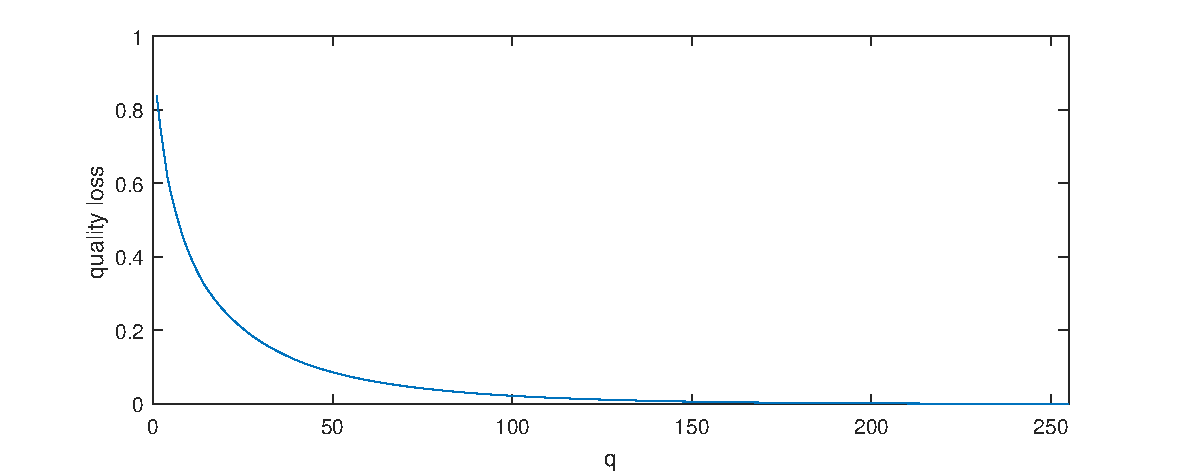
\includegraphics[width=\linewidth]{img/ThreesQualityLoss.pdf}
    \caption{Quality loss as a function of $q$. The loss drops rapidly for small values of $q$.}
    \label{fig:ThreesQualityLoss}
\end{figure}

\autoref{fig:ThreesReconstructed} shows a reconstructed handwritten three using various values of $q$. Even if the data is reduced to a single dimension, the three can still be recognized clearly.

\begin{figure}[ht]
    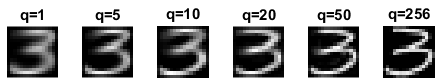
\includegraphics[width=\linewidth]{img/ThreesReconstructed.png}
    \caption{A handwritten three reduced by PCA using various values of $q$ and then reconstructed.}
    \label{fig:ThreesReconstructed}
\end{figure}

The reconstruction quality can also be determined experimentally using for example the Root Mean Square Error (RMSE). The results are shown in \autoref{fig:ThreesError}. Unsurprisingly, this function follows a trend very similar to the quality loss function. What is surprising, is that while the quality loss converges to zero, the RMSE does not. This can be explained by numerical errors in the covariance and eigenvalue calculations due to the limited precision of floating point numbers on computer hardware.

\begin{figure}[ht]
    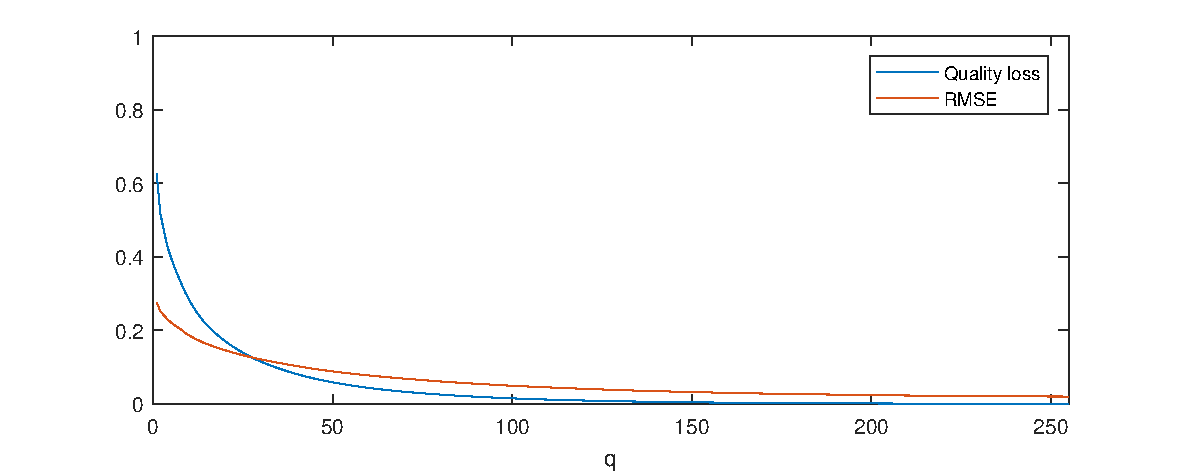
\includegraphics[width=\linewidth]{img/ThreesError.pdf}
    \caption{RMSE as a function of $q$. For comparison, the quality loss function is plotted once more.}
    \label{fig:ThreesError}
\end{figure}

\subsection{Competitive learning with SOM’s}

Self-Organizing Maps (SOMs) are a very different unsupervised technique that can (among others) serve a similar purpose as PCA: dimensionality reduction. A set of neurons is initially organized according to a specific topology (e.g. in a hexagonal grid, a square grid or random) in a space of given dimensions (typically 2D or 3D). During the training phase, the neurons are iteratively moved (so to speak) by updating their weights to the locations of the given samples. Note that the samples can optionally live in a higher dimensional space than the initial topology. In the end, the neurons should converge to new positions that fit the training data well. The network now represents a map from the original neuron locations (i.e. the prototypes) to the new locations. By considering the inverse of this map, this technique can be used to map samples in high dimensions back to a place on a potentially lower dimensional grid. Additionally, because a distance metric is defined, the distance between neurons can provide insight into the distribution and density of the training samples. This forms the basis of another application of SOMs: clustering. Each prototype represents one cluster. If the network fits a given sample to this prototype it belongs to that cluster. In this regard SOMs function very similarly to more conventional techniques such as k-means.

In a first experiment, a small $5 \times 5$ hexagonal grid of prototypes is fitted to a hollow cylinder in 100 epochs. The initial grid is always tangential to the cylinder along its main axis but not fixed to one specific side. Regardless of this variation, the final positions of the neurons are always on the inside of the cylinder, spanning most of its height. The same effects shows for similar point configurations such as hollow spheres, hollow boxes and even toroids. One possible explanation is that during the first iterations - due to the large initial neighbourhood - all neurons converge towards the center of gravity of the point cloud. However, with each iteration the neighbourhood shrinks, so in later iterations neurons start fitting more tightly to their close neighbouring points. Using other topologies or other distance functions does not change this fact. However, changing the distance function does have an effect on the initial grid topology. For example, \texttt{mandist} reduces the number of connections in hexagonal and random grids, but not in square grids. On the other hand, \texttt{boxdist} causes diagonal connections in square grids.

When the size of the prototype grid increases, the neurons start fitting better to the whole point cloud, not just the inner edges. A good rule of thumb is to use $5 \sqrt{p}$ neurons for $p$ points. The hollow cylinder consists of about 2000 points, so 225 neurons in a $15 \times 15$ grid would be ideal. In this configuration, the neurons nicely converge to the inside of the hollow cylinder body.

A small 3D initial grid (e.g. $3 \times 3 \times 3$) is also possible, although this makes the network interpretation more complex. There is also no dimensionality reduction anymore. 3D grids seem to converge in the same way as 2D grids, i.e. to the inner edge of hollow structures.

In a second experiment, the clustering capabilities of SOMs are tested on the well known Fisher's Iris flower data set. This data set contains multiple measurements of widths and lengths of both petals and sepals for three distinct Iris species. By mapping a three neuron grid onto the 4D data, clusters can be found that correspond to the three species. The adjusted rand index (ARI) function will be used to compare the SOM clustering to the species clustering and evaluate the result.

Testing all possible combinations of topology functions and distance functions did not yield any interesting results; the performance of all networks was very similar. The optimal median ARI of 0.64 was reached at 100 epochs. After only 50 epochs, the ARI was already 0.55. Both 200 and 500 epochs resulted in the exact same median ARI of 0.59 (and also the same standard deviation), so clearly the network had fully converged at this point. Since the ARI decreased again with additional epochs, this could be a sign of overfitting.

\section{Deep learning}
\subsection{Digit Classification with Stacked Autoencoders}
While classic techniques such as PCA to reduce the dimensionality of input data work fine, deep neural nets offer an interesting alternative. Stacked autoencoders manage to reduce the dimensionality using common neural network training schemes.

Here, the accuracy of stacked autoencoders is tested in the context of digit classification and compared to that of traditional (non-deep) neural networks. The stacked autoencoders is first trained greedily, layer by layer. Next, the whole stack is further finetuned using regular training. Important parameters in this process are the number of hidden layers, the number of hidden neurons in each layer and the maximum number of epochs.

The methodology used is similar to that in earlier exercises: vary some important parameters, train a stacked autoencoder using these settings repeatedly (i.e. twice instead of the regular ten times due to long calculation times), and store the results in terms of training time and accuracy. The number of hidden neurons in the last layer is either 20, 50 or 100. That number doubles with every preceding layer. The possible \texttt{MaxEpoch} settings used in the first hidden layer are 4, 40, 60 and 100. In the middle hidden layer (in case of a 4 layer network) those values are divided by two, while in the last hidden layer they are divided by four. The output layer uses double those of the first layer.

In a stacked autoencoder with two hidden layers the results were very similar for a wide range of input parameters. Configurations with the smallest \texttt{MaxEpoch} settings resulted in accuracies in the range of 80\% to 90\%. All other \texttt{MaxEpoch} settings produced accuracies between 98.66\% and 99.70\% regardless of network architecture. Less than ten epochs was thus not enough for the network to fully convergence. The training time taken for each trial fell between 27.5s for small networks using few epochs to 118.0s for the largest networks using the maximum number of epochs. A stacked autoencoder with three hidden layers was also tested using the same methodology. The results from this experiment were very similar: a maximum accuracy of 99.72\%. Since the performance is not significantly better, the simpler autoencoder is preferred.

The results of the stacked autoencoders were compared to those of two classic (i.e. non-deep) neural networks created with the \texttt{patternnet} MATLAB function. One has a single hidden layer of size 100 and another has two hidden layers of sizes 100 and 50. Optimizing these networks is beyond the scope of this exercise, so default parameters were used. In the past exercises these default parameters have proven to be good choices nonetheless. The network with a single hidden layer achieved a maximum accuracy of 97.64\% over ten trial runs. The network with two hidden layers reached 97.88\%. Both values are lower than the worst accuracy of a stacked autoencoder performing the same task (after sufficient epochs). On the other hand, both take a lot less time to train: the median durations over ten trial runs were 14.5s and 15.8s respectively.

\subsection{Convolutional Neural Networks}
In this exercise a pre-trained Convolutional Neural Network (CNN) is used to classify images as either an airplane, a ferry or a laptop. The input layer accepts images of size 227px $\times$ 227px. The images must contain three color channels: red, green and blue. The second layer is a convolutional layer with weights of size $11 \times 11 \times 3 \times 96$. This means there are 96 convolution masks of size $11 \times 11 \times 3$ (where the 3 corresponds to the three color channels). Each of these masks will be convolved with the image using a certain stride ($[4, 4]$ in this case). Every step in the convolution results in a single value that is assigned to a pixel in the output of the layer. Since there is no stride value for the depth (i.e. colors), these are presumably all compressed into one dimension. It is also presumed that convolution starts at pixel $(1, 1)$ and that parts of the mask outside the image can be handled appropriately. Alternatively, it could also start at pixel $(6, 6)$ so that the mask is never outside of the image, but this would reduce the resulting image size even with stride $[1, 1]$. In conclusion, the second layer will output 96 2D images (one for each mask) with sizes of approximately $\frac{227}{4} \times \frac{227}{4} \approx 56 \times 56$. 

Layers three (ReLu) and four (normalization) do not change these dimensions.

Layer five is a max pooling layer of size $3 \times 3$ using stride $[2 2]$. This means the 96 images are halved in each dimension once more to $28 \times 28$.

The last fully connected layer contains 1000 neurons since this network was pre-trained to classify images in 1000 different classes. However, in our case, only three are really used. Regardless, this is a huge reduction considering that the problem started from images with dimensionality $227 \times 227 \times 3 = 154 587$ pixels using 8 bits per pixel. 

\section{Nonlinear regression and classification with MLPs}
\subsection{Regression}
\label{ssec:p1_regression}

The goal of this exercise is to approximate a function $f(X_1, X_2)$ using MLPs. This function is a linear combination of five base functions; more specifically $f(X_1, X_2) = \frac{1}{18}(9f_1(X_1, X_2) + 4f_2(X_1, X_2) + 4f_3(X_1, X_2) + f_4(X_1, X_2) + 0f_5(X_1, X_2))$. The equations that determine these five base functions are unknown, but 13 600 noise-free points are given for each function. All base functions are continuous and most contain strong sinusoidal patterns in both the $X_1$ and $X_2$ direction.

\begin{figure}[ht]
    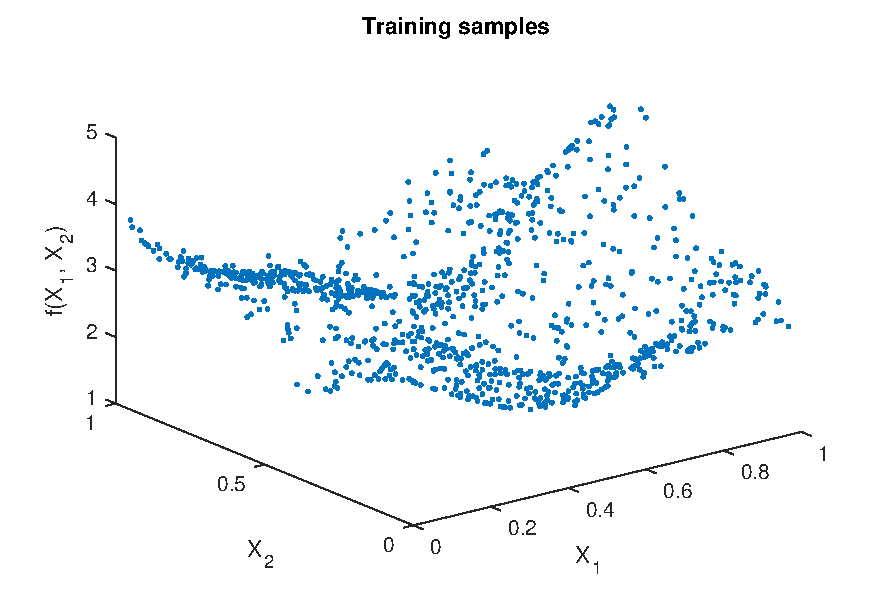
\includegraphics[width=\linewidth]{img/TrainPoints.pdf}
    \caption{1 000 randomly selected training samples from all given points that make up $f$.}
    \label{fig:TrainPoints}
\end{figure}

% \begin{figure*}[t]
%     \begin{subfigure}{0.49\linewidth}
%         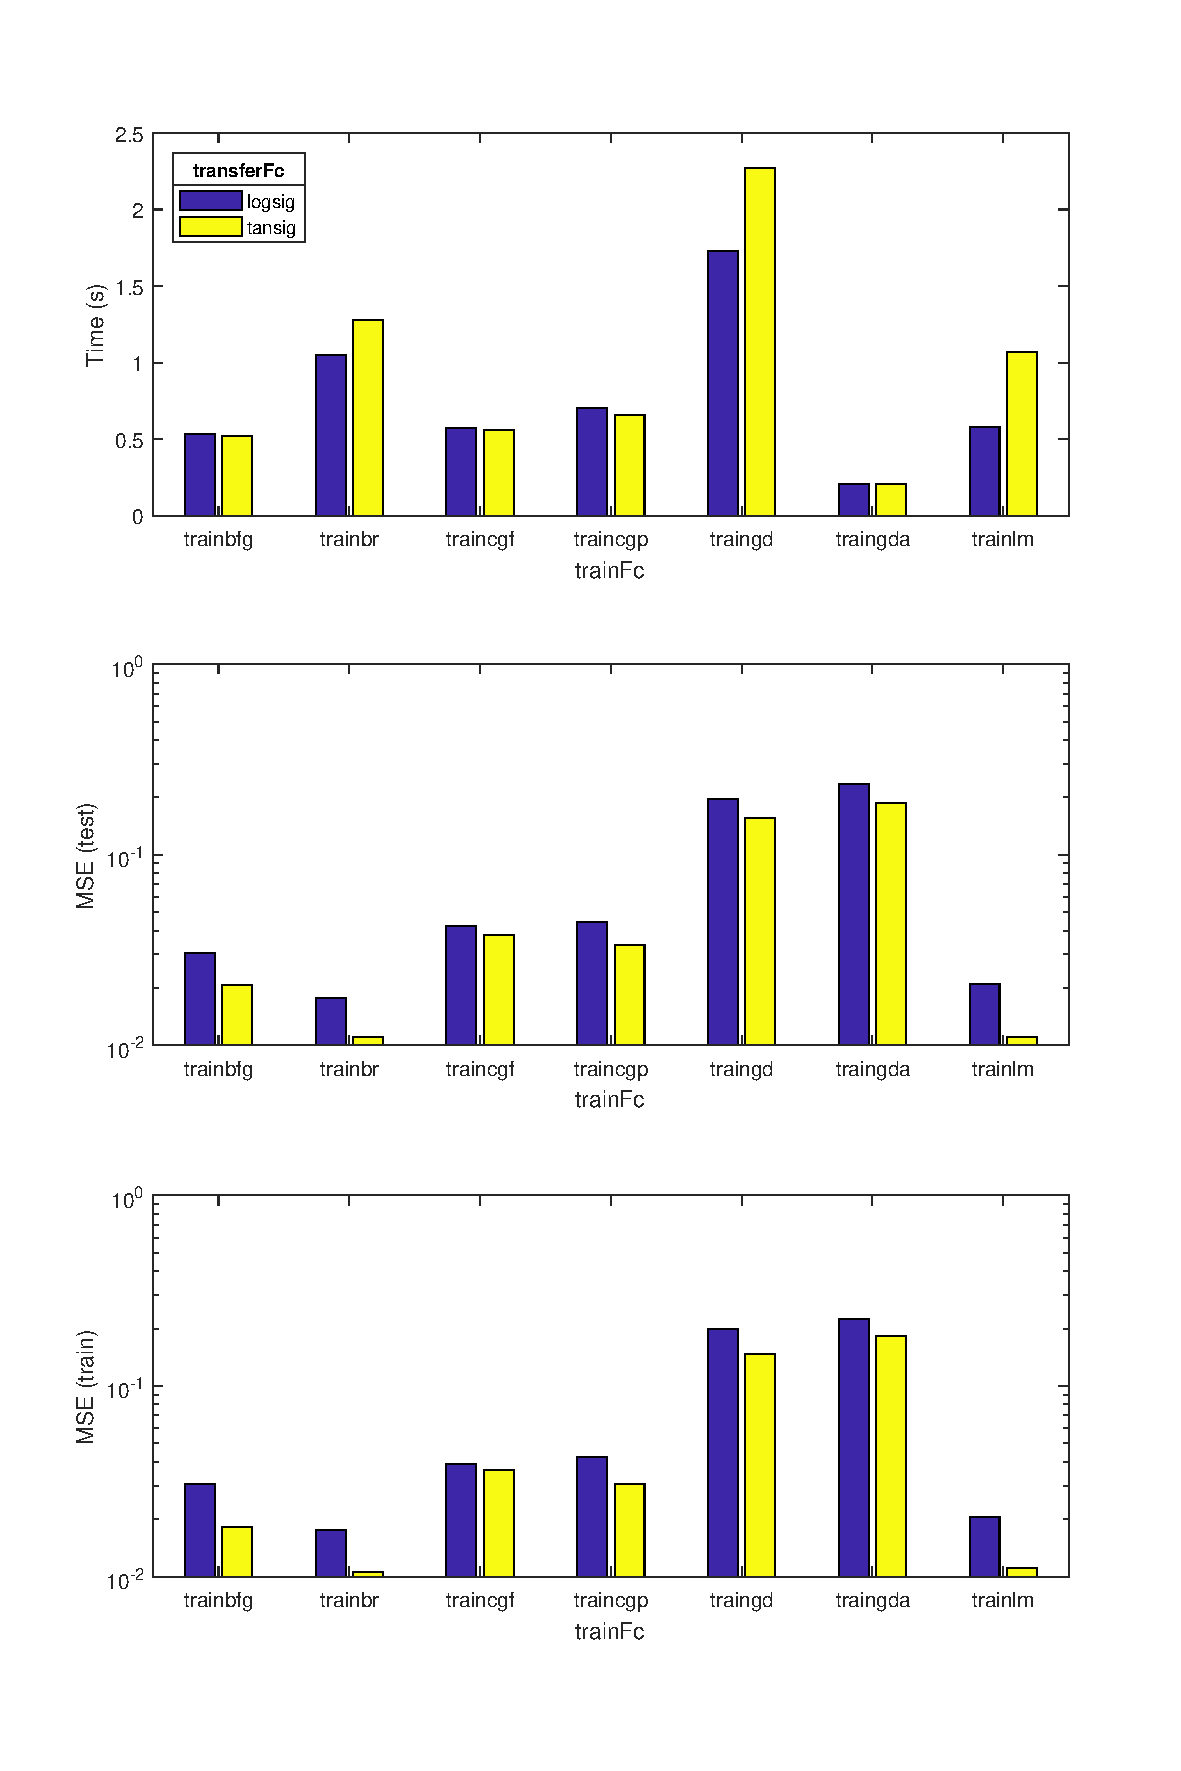
\includegraphics[width=\linewidth]{img/Regression_transferFc.pdf}
%         \caption{Transfer functions compared}
%     \end{subfigure}
%     \begin{subfigure}{0.49\linewidth}
%         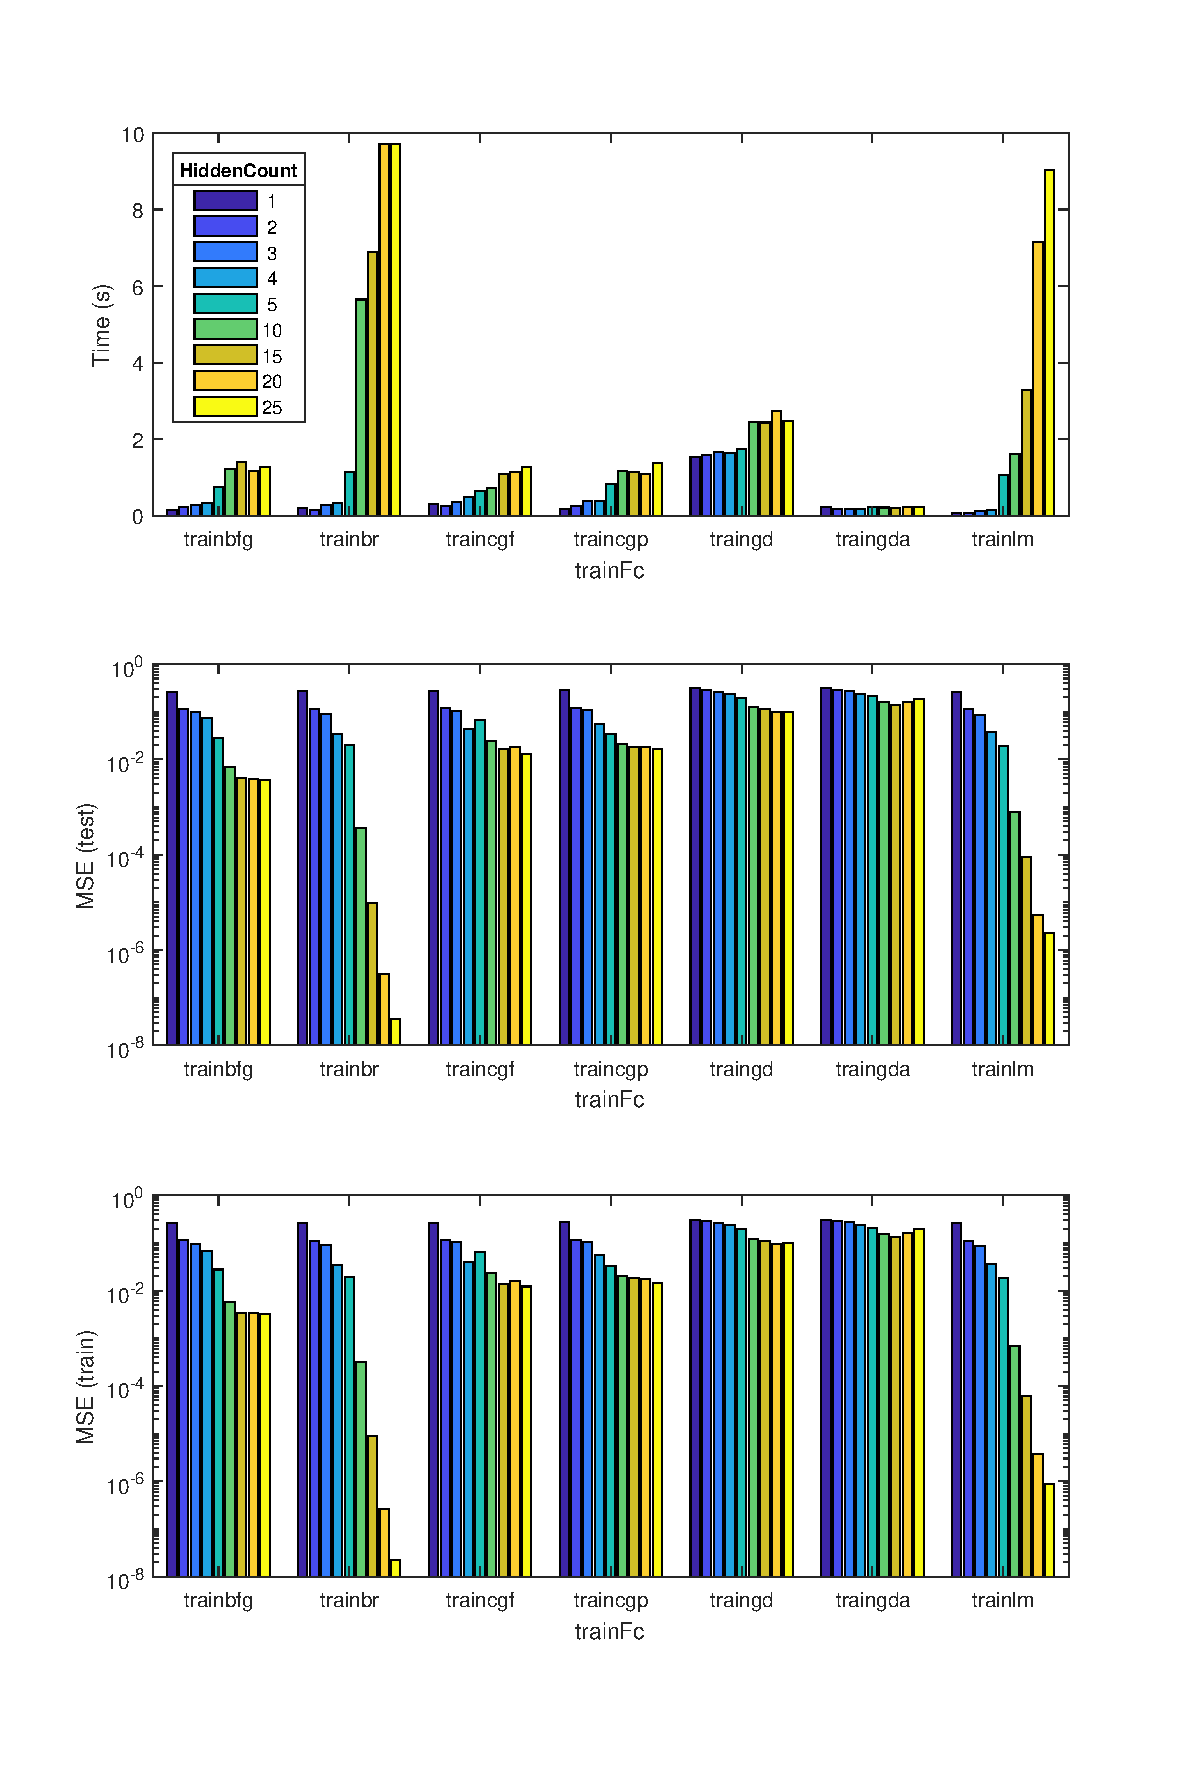
\includegraphics[width=\linewidth]{img/Regression_HiddenCount.pdf}
%         \caption{Network architectures compared}
%     \end{subfigure}
%      \caption{Performance of various training functions for the regression task in terms of median training time and MSE on both the train and test set.}
%     \label{fig:Regression_Perf}
% \end{figure*}

Before training the MLP, 3 000 samples are selected from all given points - 1 000 each for training, validation and testing. These sample sets should ideally be independent. Selecting all points in a small neighbourhood as sample set is not a good idea because this way only a small portion of the whole function domain is sampled. Selecting points on a fixed stride is also a bad idea because sinusoidal functions are periodic and this could once more promote strong correlation between samples. On the other hand, samples gathered through this approach will cover the whole function domain. Instead, the samples will be selected at random from all given points to maximize independentness. \autoref{fig:TrainPoints} shows a random selection of 1 000 training samples from all given points.

As usual, the network architecture is kept as simple as possible. This means only one hidden layer is used. The number of neurons in this layer will be varied and the results of each architecture will be compared. Multiple learning functions will be evaluated. The effect of the choice of transfer function in the hidden layer will also be tested. However, the transfer function in the output layer will always be the default (\texttt{purelin}) since this is a regression task and as such a continuous output value is required. Other settings that are not explicitly mentioned will also remain at their default value. Each test will be repeated ten times and median values will be reported.

To assess the performance of a certain configuration, both training time and accuracy are taken into account. Accuracy (or lack thereof) is measured as Mean Squared Error (MSE). The results are shown in \autoref{fig:Regression_Perf}. In terms of transfer function in the hidden layer (graph omitted), the results are similar for both \texttt{logsig} and \texttt{tansig}. For most training functions, the former is slightly faster while the latter scores slightly better in terms of MSE. The real performance differences are caused by the training functions and the network architecture choices. \texttt{trainlm} once more performs very well, but this time it is bested by \texttt{trainbr}. For networks with a limited amount of hidden neurons they perform very similar, but the latter keeps improving when more hidden neurons are added. Both training functions do take a long time to reach a low MSE. Finally, note how the MSE is very similar for both train and test sets. The train set does slightly better in general because it is actively being optimized, while the test set just follows along.

\begin{figure}[ht]
    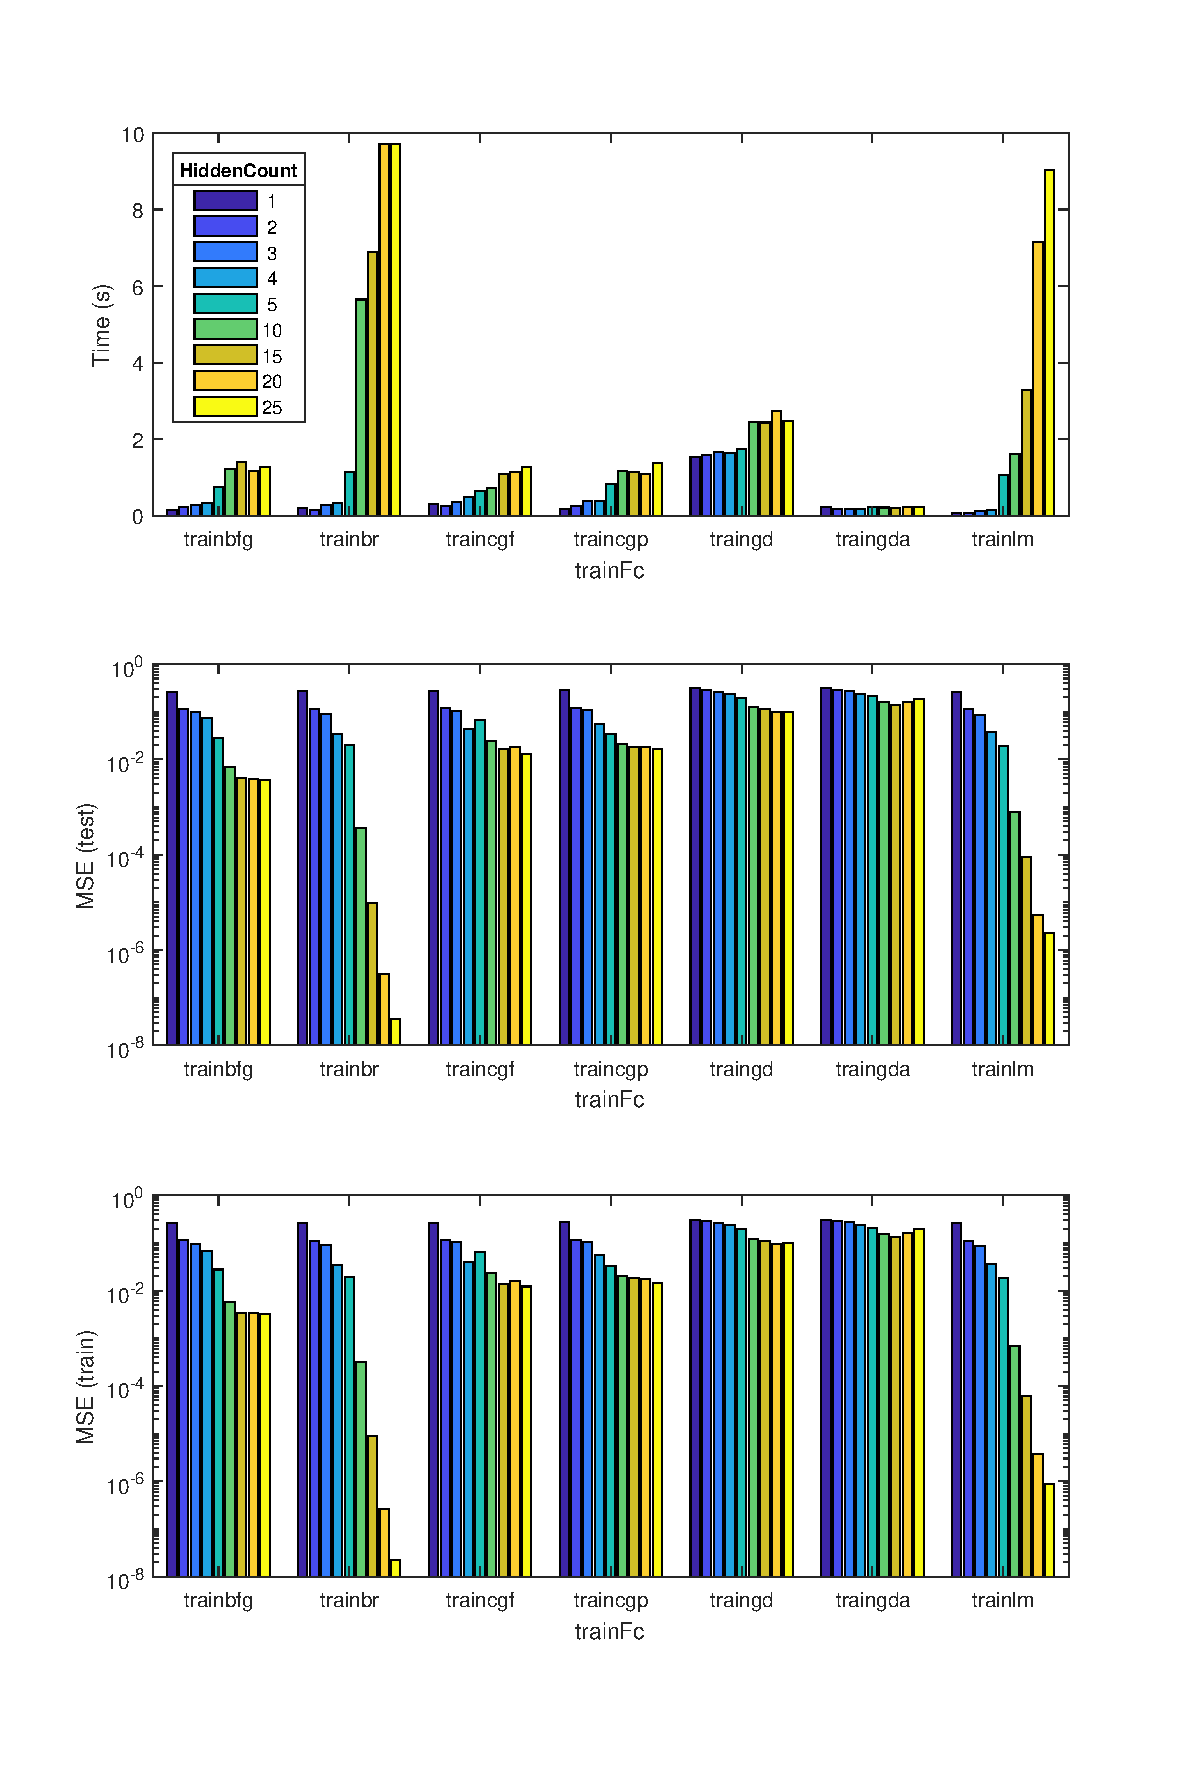
\includegraphics[width=\linewidth]{img/Regression_HiddenCount.pdf}
     \caption{Performance of various training functions for the regression task in terms of median training time and MSE on both the train and test set.}
    \label{fig:Regression_Perf}
\end{figure}

For the remainder of this section, we will only use the best configuration: a network with 25 hidden neurons, \texttt{tansig} as transfer function in the hidden layer and training functions \texttt{trainbr}. In this configuration, validation checks are disabled by default. This causes the algorithm to always use the maximum number of epochs, which takes time. \autoref{fig:Regression_trainbr_Perf} shows that the validation error decreases monotonically together with the train and test error, so enabling validation would not have made a difference (except for some calculation overhead). A plot of the test set and the network approximation thereof is omitted from this report because both plots are visually indistinguishable from each other and very similar to \autoref{fig:TrainPoints}.

\begin{figure}[ht]
    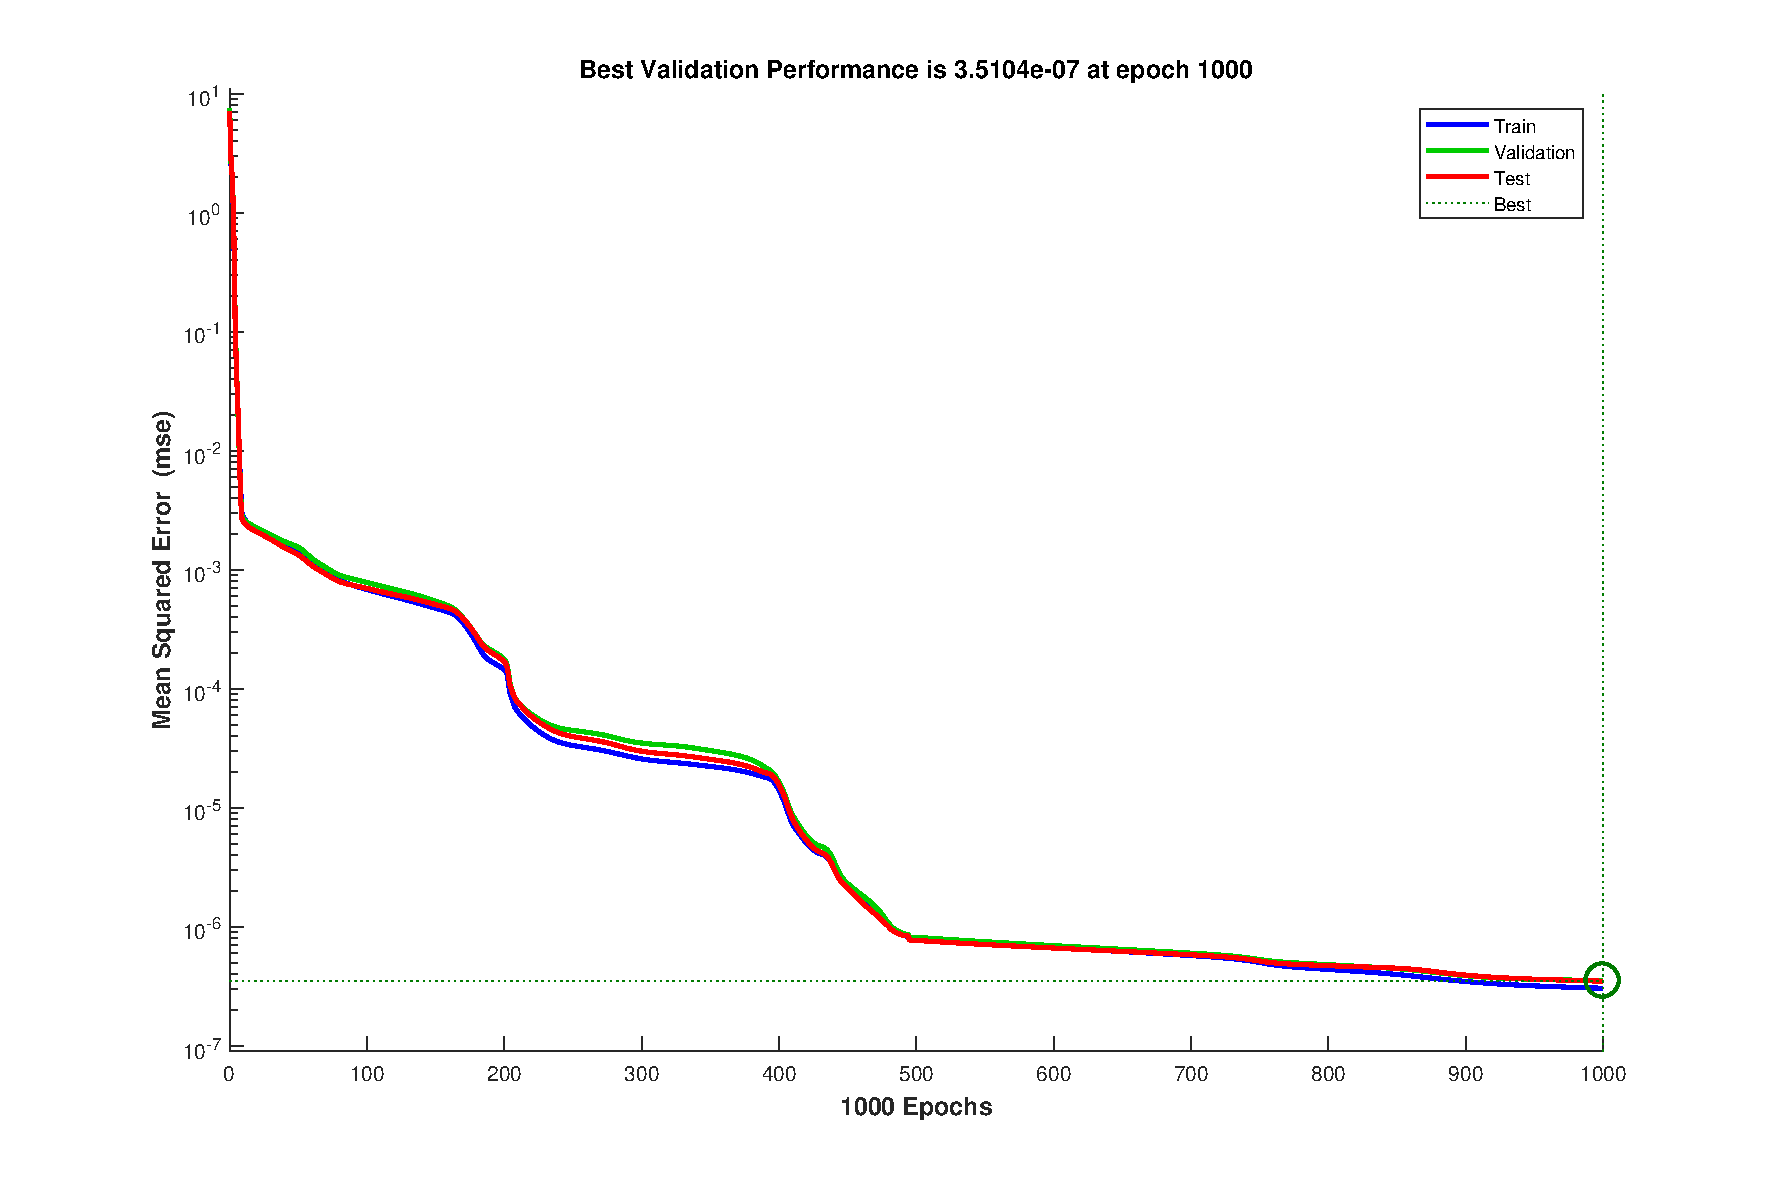
\includegraphics[width=\linewidth]{img/Regression_trainbr_Perf.pdf}
    \caption{Error curves for \texttt{trainbr}. All three curves decrease monotonically and have apparently not yet reached their minimum after 1000 epochs.}
    \label{fig:Regression_trainbr_Perf}
\end{figure}

The MSE of this network can be reduced even further by increasing the number of hidden neurons or the maximum amount of epochs, both at the cost of more training time. However, at 25 hidden neurons and 1000 epochs, the network approximations are already barely distinguishable from the original. If other training functions were used, their hyperparameters could be optimized using another grid search, but that happens automatically in the case of \texttt{trainbr}.

\subsection{Classification}
While the previous exercise focussed on regression, MLPs can also be used to for classification tasks. More specifically, the goal is to create a binary classifier that can distinguish between two classes (quality 5 and quality 6) of white wine using the dataset from Cortez et al. \cite{cortez2009modeling}. When assessing the performance of the solution, keep in mind that the quality scores of both classes are very close and that assessing wine quality is a subjective endeavor.

The network architectures that will be tested are the same as those in \autoref{ssec:p1_regression}. The single difference is the output layer. One output neuron per class will be used instead of just one output neuron in general. The transfer function \texttt{softmax} will be used and the neuron with the highest output value wins. Alternatively, a classification problem can also be seen as a regression problem where the goal is to approximate the class label. In that case, a single output neuron suffices. In the following experiments, only the first approach is used. On top of the classic training functions we used in previous exercises, two extra training functions will be evaluated for this classification task: \texttt{trainscg} and \texttt{trainrp}. The neural network will be evaluated based on the Correct Classification Ratio (CCR): the percentage of correctly classified samples (i.e. the accuracy). 

% Because the number of samples is both classes is reasonably balanced (1457 vs. 2198 samples), this metric is a decent indicator of performance. The CCR is not used as a performance function for the neural network during training. Instead, a cross-entropy score is used. This score takes the underlying predicted probabilities into account, and penalizes small errors that flip the predicted class less than the accuracy score would.

The results show that the choice of transfer function in the hidden layer (\texttt{tansig} or \texttt{logsig}) did not affect the CCR or training time in a significant way. Remarkably, the training function did not affect the CCR very much either. \autoref{fig:WineResults} shows that most algorithms result in a neural network that reaches a CCR of about 70\%. As expected, plain gradient descent (\texttt{traingd}) does worst and takes a very long time while \texttt{trainlm} does slightly better than average.

\begin{figure*}[t]
    \begin{subfigure}{0.49\linewidth}
        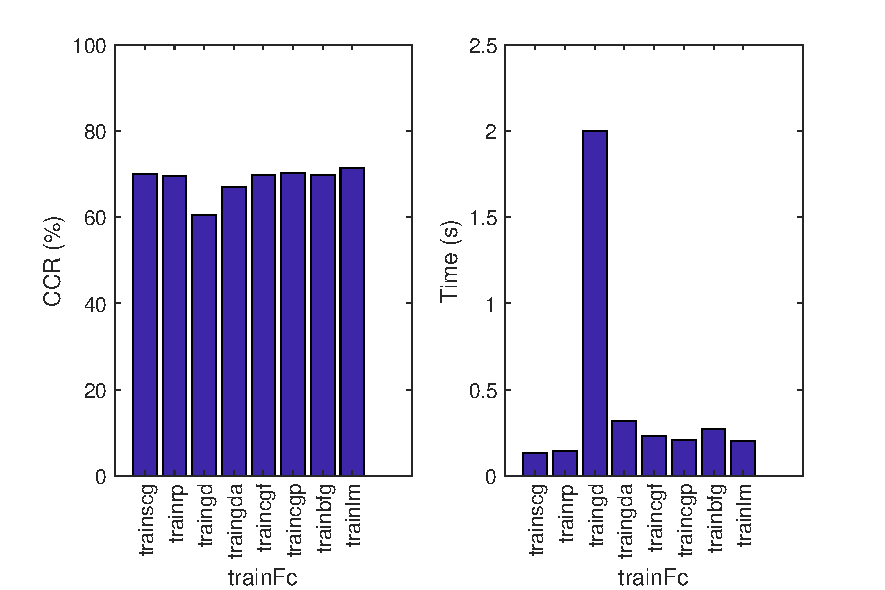
\includegraphics[width=\linewidth]{img/WineResults.pdf}
        \caption{Training functions compared}
        \label{fig:WineResults}
    \end{subfigure}
    \begin{subfigure}{0.49\linewidth}
        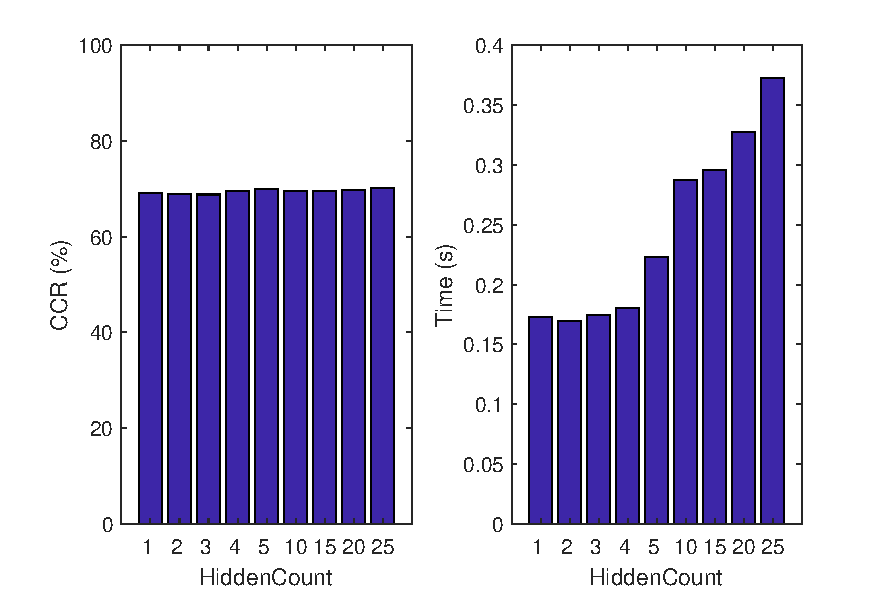
\includegraphics[width=\linewidth]{img/WineResultsArch.pdf}
        \caption{Network architectures compared}
        \label{fig:WineResultsArch}
    \end{subfigure}
     \caption{Median CCR and training time of various configurations.}
\end{figure*}

\autoref{fig:WineResultsArch} shows that even changes in the network architecture do not change the CCR significantly. Of course a higher number of neurons implies more calculations and thus a longer training time. More extreme architectures with hundreds of neurons were also tested, but the results were identical. Next, more hidden layers were introduced (up to ten). This could allow the network to define more complex decision boundaries. Unfortunately, there was no performance improvement.

To investigate why the CCR always remains around 70\%, a better understanding of the training data is needed. There are eleven input columns, which makes it hard to visualize this dataset. However, if there is some correlation between the columns of our data set, that fact can be exploited by applying PCA before training. If the essence can be summarized in three dimensions or less, the reduced dataset can be visualized properly. Applying PCA also reduces the number of computations and should thus speed up the training process. The normalized cumulative sum of the $q$ largest eigenvalues gives a good indication of the quality that can be expected of a dimensionality reduction to $q$ columns. In \autoref{fig:WineQualityLoss}, the theoretical quality loss is plotted with respect to $q$. Clearly, there is much redundancy in our columns because there is hardly any quality loss by going from eleven to three columns.

\begin{figure}[ht]
    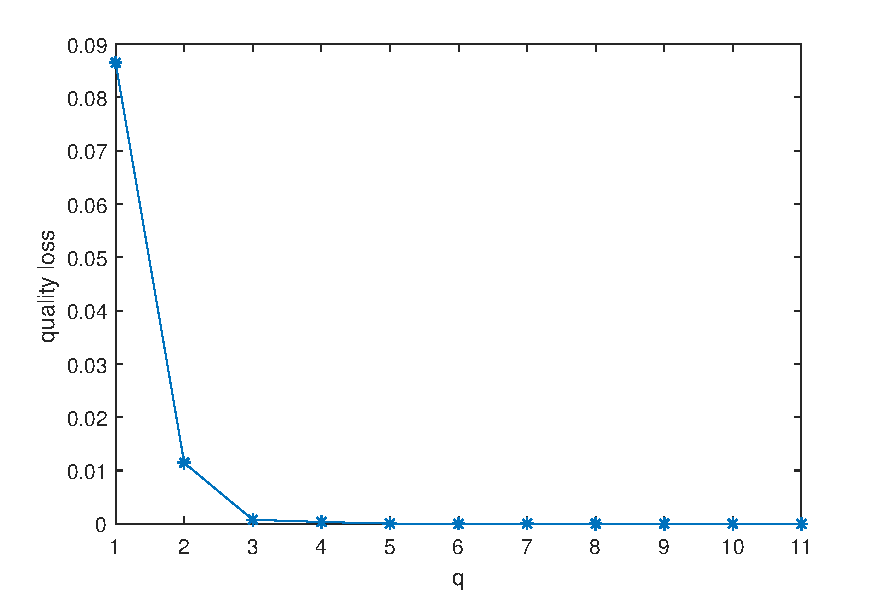
\includegraphics[width=\linewidth]{img/WineQualityLoss.pdf}
    \caption{The loss of quality when reducing the dimensionality to $q$ with PCA. Almost all relevant information is captured by the three largest principal components.}
    \label{fig:WineQualityLoss}
\end{figure}

The quality does not tell the whole story. After applying PCA with $q=3$, the Root Mean Squared Error (RMSE) tells us exactly how good the reconstruction is. On average over all columns the normalized RMSE is 0.67, but it ranges from 0.40 to 0.95. In absolute values the differences are much bigger because some columns contain rather large values (e.g. TotalSulfurDioxide) while others only contain small values (e.g. VolatileAcidity). Contrary to what the PCA quality predicted, these errors are quite large. They can be reduced by choosing a higher value of $q$. However, in the remainder of this section $q=3$ so that the data can be visualized directly.

Such a visualization in shown in \autoref{fig:WinePrediction}. Along the three largest principal components, there is no clear boundary between the two quality classes. Regions exist where one class is more prominent than the other, but the effect is rather subtle. In the same image, we see how a neural network with default parameters learns from such data and attempts to find a decision boundary. The result is a quasi-linear cut through the 3D space. Clearly this network avoided overfitting at all costs, preferring a large bias in return for low variance. This can also be seen during the training phase: the training algorithm regularly checks the performance of a separate validation set. If this performance degrades significantly, a validation error is triggered. Such validation errors happen often when using the wine data set, causing the algorithm to stop long before the maximum number of epochs is reached. Increasing the validation error threshold enables the algorithm to run for more epochs, but our tests show that this does not result in a higher accuracy. In other words, the training data is not consistent enough to make more accurate predictions.

\begin{figure}[ht]
    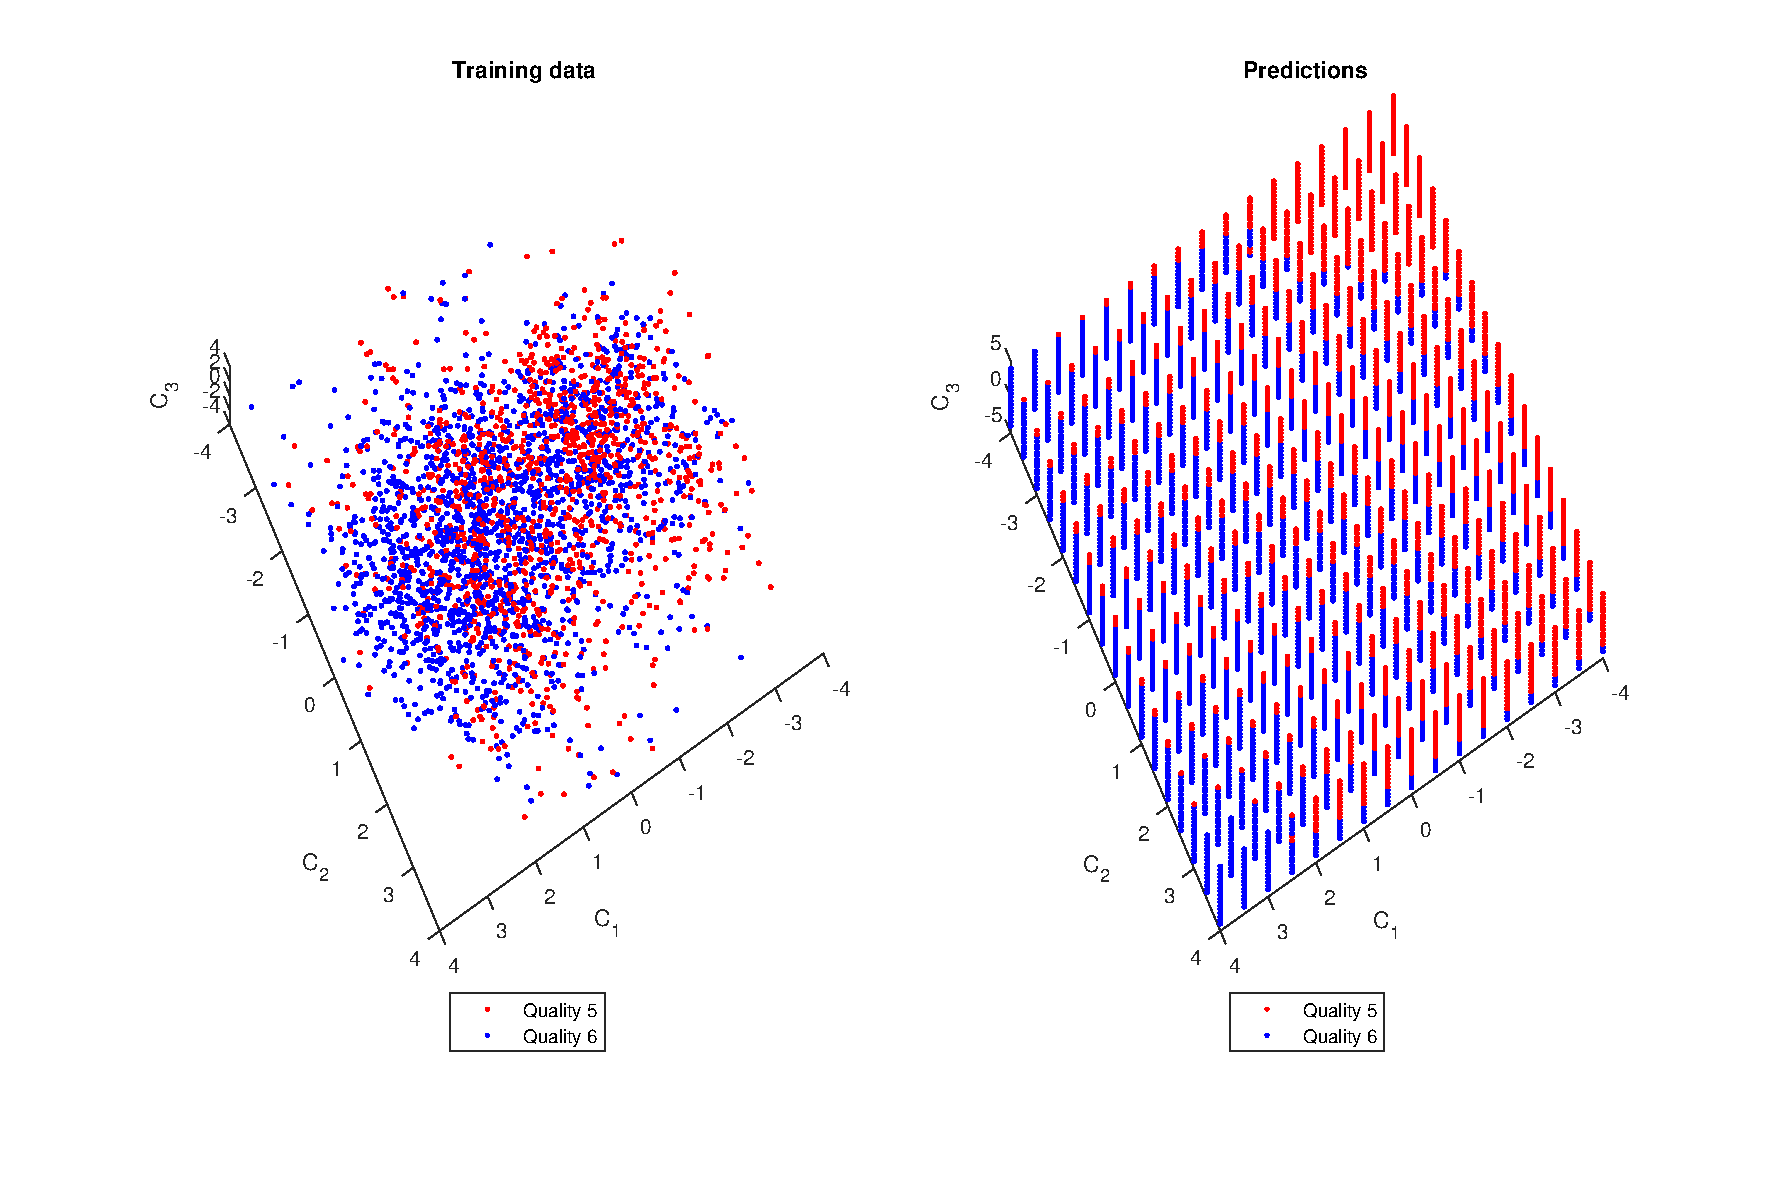
\includegraphics[width=\linewidth]{img/WinePrediction.pdf}
    \caption{The left plot shows the distribution of the two quality classes in the reduced space. The right plot shows predictions of a neural network trained on the reduced training data for the whole 3D space.}
    \label{fig:WinePrediction}
\end{figure}

The tests regarding network architecture and training function that have been performed without PCA are now repeated on the same samples after PCA dimensionality reduction. Since the RMSE values of the reconstruction were quite large, the accuracy is expected to be lower than before but the other conclusions should remain the same. \autoref{fig:WineResultsPCA} and \autoref{fig:WineResultsArchPCA} summarize the results.

\begin{figure*}[t]
    \begin{subfigure}{0.49\linewidth}
        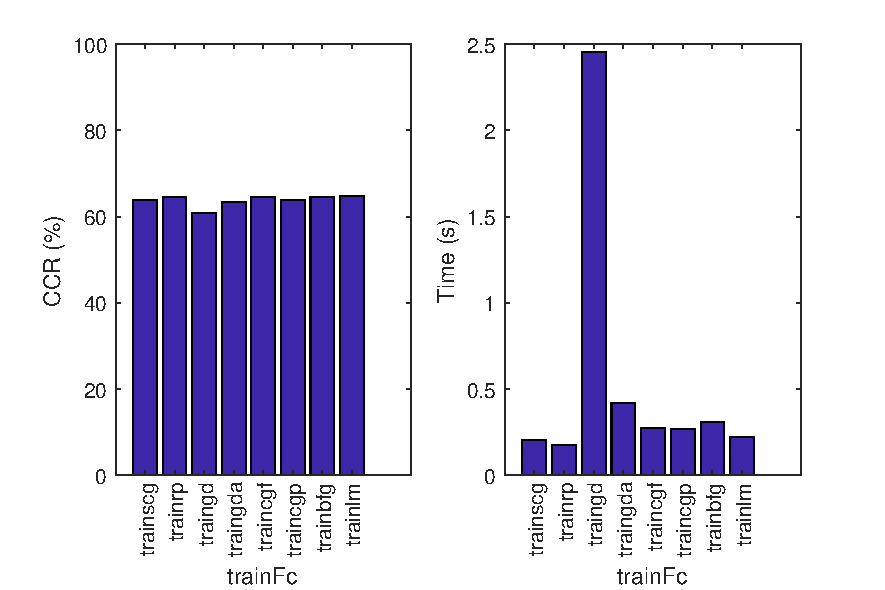
\includegraphics[width=\linewidth]{img/WineResultsPCA.pdf}
        \caption{Training functions compared}
        \label{fig:WineResultsPCA}
    \end{subfigure}
    \begin{subfigure}{0.49\linewidth}
        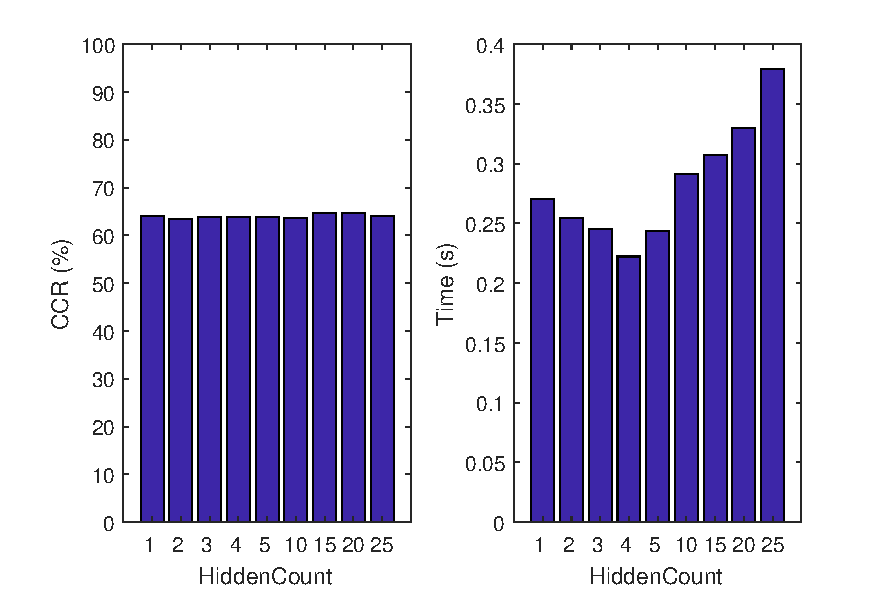
\includegraphics[width=\linewidth]{img/WineResultsArchPCA.pdf}
        \caption{Network architectures compared}
        \label{fig:WineResultsArchPCA}
    \end{subfigure}
     \caption{Median CCR and training time of various configurations after applying PCA with $q=3$.}
\end{figure*}

As expected, the results follow the same patterns as before. The CCR is consistent accross training functions and network architectures, albeit lower than before. The training duration also follows a similar pattern with gradient descent being notoriously slow once more. It is remarkable that training (excluding PCA preprocessing) appears slower than before, even though less data had to be processed. Perhaps the reduction from eleven to three is not enough to make much of a difference. Also remarkable is that the training time drops every time an extra hidden neuron is added - up to four hidden neurons at least. Keep in mind that the classic tic/toc MATLAB time measurement methodology that generated these results is not very reliable and did not happen in a tightly controlled environment, so no strong conclusions can be drawn from these results.

In conclusion, PCA is useful in this case if it can reduce the dimensionality of the samples to three dimensions or less. That way, the data can be properly visualized. However, PCA does not seem to speed up the training phase and it lowers the accuracy due to the loss of information.

%TODO patterns in error histogram?

\section{Character recognition with Hopfield networks}

Similar to \autoref{ssec:hopfield}, the goal of this exercise is to recognize inputs corrupted by noise using a Hopfield network. While earlier targets consisted only of digits, here both lower and upper case letters are used as inputs. More specifically, $7px \times 5px$ binary images of all 33 letters in \texttt{svenahoABCDEFGHIJKLMNOPQRSTUVWQYZ} are used to train a Hopfield network. The first ten letters are shown in \autoref{fig:Letters_First10}. Each letter is represented by a vector $\xi^\mu = [\xi_1^\mu, \ldots, \xi_N^\mu]^T$ (where $N=7 \times 5=35$ and $\xi_i^\mu \in \{-1, +1\}$) with the same bits as the image. The resulting network will consequently consist of $N$ neurons.

\begin{figure}[ht]
    
\includegraphics[width=\linewidth]{img/Letters_First10.png}
    \caption{The first 10 of 33 letters used as training data for the Hopfield network.}
    \label{fig:Letters_First10}
\end{figure}

First, the network is trained on the a selection $S_P = \{\xi^\mu\}_{\mu=1}^P$ (where $1 \leq P \leq 33$) of the 33 clean input vectors. Training here means setting the interconnection weights of the neurons according to the Hebb rule: $w_{ij} = \frac{1}{N} \sum_{\mu=1}^{P}\xi_i^\mu \xi_j^\mu$. Next, the vectors in that selection are corrupted by flipping three random bits in each of them. The corrupted selection is given as input to the network. Ideally, the output of the network after $I$ iterations equals the clean version of the input. Unfortunately that is not always the case, for example because the calculations have not converged yet or because a spurious attractor is involved. Even in the absense of spurious attractors, perfect convergence can take a while. To speed up the process, the decimal numbers in the output are rounded to the nearest binary state. The error after rounding is defined as the number of bits that differ between input and output over all vectors in the selection $S_P$.

Hopfield networks have a property called the Critical Loading Capacity (CLC). This is the number of vectors $P_{max}$ that can be stored in the network and then recalled again without error. The probability of errors depends on both $N$ and $P$ (and $I$). For large $P$ and $N$ and the error probability close to zero, $\frac{P}{N} \approx 0.138$, so more patterns need to be compensated for with extra neurons to keep the error probability stable.

To determine the CLC of the network in practise, the error after rounding is determined for all selections $S_P$ with $P=1..33$. For small values of P the error is expected to be zero because the CLC has not been reached. When P surpasses the CLC, the error will start rising sharply. Experiments confirm this, as shown in \autoref{fig:Letters_SinglePerf}. Each individual test was performed ten times and the median error value was plotted. Not only $P$, but also the number of iterations $I$ has an effect on the error. Note that more iterations were only attempted if the current amount of iterations resulted in at least one error.

\begin{figure}[ht]
    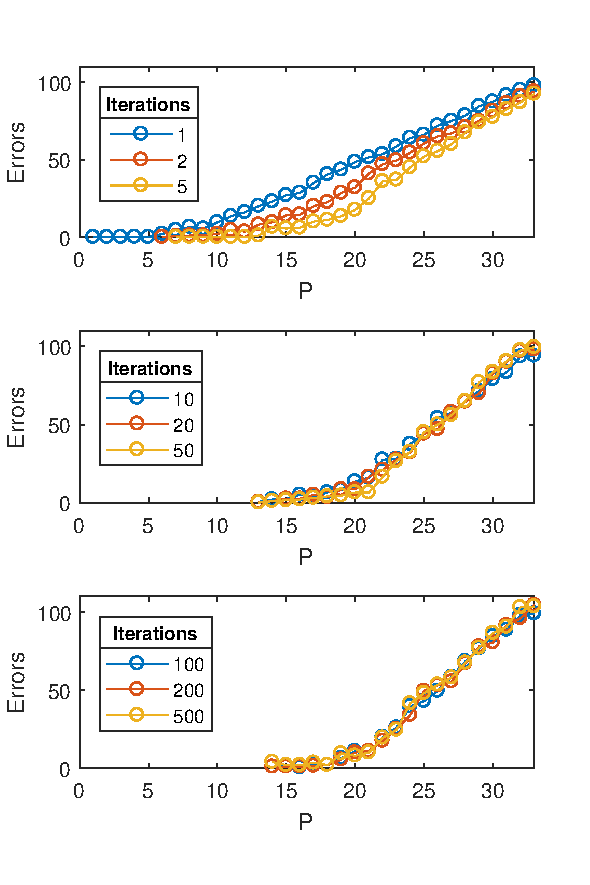
\includegraphics[width=\linewidth]{img/Letters_SinglePerf.pdf}
    \caption{The error after rounding in function of selection size $P$ for various numbers of iterations $I$.}
    \label{fig:Letters_SinglePerf}
\end{figure}

When fewer than six vectors are stored in the network, a single iteration is often enough to retrieve the correct letter. When more vectors are added, more iterations are needed to avoid errors. Since the network converges after a number of iterations, this method to raise the loading capacity has its limits. It is better to think of the CLC as the number of vectors that can be stored and recalled without error after enough iterations so that the network has converged. Since the differences between 100, 200 and 500 iterations cannot be made out anymore on the plot, the network is considered to be converged after 100 iterations. The CLC $P_{max}$ then equals 14. Note that this value is larger than the theoretical CLC of $0.138 \times N \approx 5$. The difference is due to the experimental setup involving the median error of ten trials. This median is zero only if at least six in ten error counts were zero. However, the corresponding error probability is still higher than the probability used to calculate the $0.138$ factor. In other words, the used experimental setup is more tolerant towards errors and as such the $\frac{P}{N}$ ratio is higher.

To store and recall more than 14 patterns without error using this methodology, other tricks must be used. The most straightforward trick involves increasing the number of neurons $N$ in the Hopfield network. This number is determined by the length of the input vectors during training. The vector length in turn is determined by the number of pixels in the original image. One option then is to use higher resolution bitmaps, but that is not feasible in this exercise. Instead, the extra bits in the vector can be filled uniformly with plus or minus one. Note that this would place all vectors in one particular corner of the high dimensional space. Since vector proximity is a source of potential error in Hopfield networks, this is best avoided. The extra bits can also be filled randomly. This should disperse the vectors evenly over the extra dimensions. Another possibility is to simply duplicate the contents one or more times. \autoref{fig:Letters_DoublePerf} shows what happens when the image is repeated once and the vector length is consequently increased to 70.

\begin{figure}[ht]
    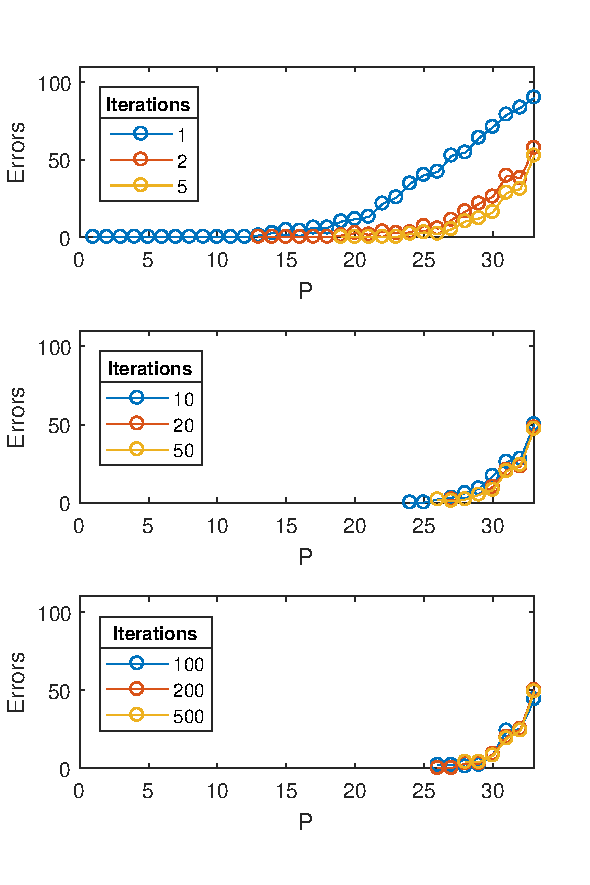
\includegraphics[width=\linewidth]{img/Letters_DoublePerf.pdf}
    \caption{The error after rounding when vectors of size $N=70$ are used.}
    \label{fig:Letters_DoublePerf}
\end{figure}

Using this method, the CLC increases to 26 when the network has fully converged. Note that $26 \approx 2 \times 14$, which makes sense since $N$ has also doubled.

A brief literature review suggests that there is another trick; one involving strong attractors \cite{edalat2013strong}. Such attractors are just like regular attractors, except that they have a certain multiplicity or degree $d_\mu > 1$. In other words, the same attractor is given as input to the network multiple times. The approximate theoretical CRC of such a strong pattern is $0.138 \times N \times d_\mu$. Instead of doubling the image size, the multiplicity of the vectors can be set to two for the same effect. Unfortunately MATLAB does not appear to support this feature. Manually  repeating the input vectors does not have the intended effect either.

For a discussion on spurious attractors, review \autoref{ssec:hopfield}. Applying the theory to this problem, the number of spurious attractors is expected to increase with the number of input vectors $P$ since more combinations of vectors become possible. However, in practice, during all experiments for this exercise not a single spurious attractor was encountered. Perhaps they could be revealed with brute force by providing many random noise samples as simulation input to the network.

\bibliographystyle{alpha}
\bibliography{references}

\clearpage
\onecolumn

\begin{appendices}

\lstset{language=Matlab,%
    %basicstyle=\color{red},
    breaklines=true,%
    morekeywords={matlab2tikz},
    keywordstyle=\color{blue},%
    morekeywords=[2]{1}, keywordstyle=[2]{\color{black}},
    identifierstyle=\color{black},%
    stringstyle=\color{mylilas},
    commentstyle=\color{mygreen},%
    showstringspaces=false,%
    numbers=left,%
    numberstyle={\tiny \color{black}},% size of the numbers
    numbersep=9pt, % this defines how far the numbers are from the text
}

%TODO MATLAB code
\section{Nonlinear regression and classification with MLPs}
\subsection{Regression}
\lstinputlisting{src/1/ffnet.m}
\lstinputlisting{src/1/test_with_plots.m}

\subsection{Classification}
\lstinputlisting{src/2/without_pca.m}
\lstinputlisting{src/2/with_pca.m}

\section{Character recognition with Hopfield networks}
\lstinputlisting{src/3/hopfield.m}
\lstinputlisting{src/3/hop_perf.m}
\lstinputlisting{src/3/distort.m}
\lstinputlisting{src/3/distortall.m}
\lstinputlisting{src/3/vec2img.m}

\end{appendices}
\end{document}